\documentclass[11pt,UTF8]{ctexart}
\usepackage{setspace}
\usepackage{geometry}
\usepackage{amsthm,amsmath,amsfonts,amssymb}%\because\therefore
\usepackage{mathtools}%underset
\usepackage{cancel}
\usepackage{extarrows}
\usepackage{enumerate}
\usepackage{tikz,tikz-cd,forest}
\usepackage{float}
\usepackage{gensymb}
\usepackage{url}
\usepackage[unicode=true,%本行非常重要 支持中文目录hyperref CJKbookmarks对二级目录没用
	colorlinks,
	linkcolor=black,
	anchorcolor=black,
	citecolor=black,
	CJKbookmarks=false]{hyperref}
\usepackage{datetime}
\newdateformat{builddatemonth}{\THEYEAR.\twodigit{\THEMONTH}}
\newdateformat{builddate}{\THEYEAR\twodigit{\THEMONTH}\twodigit{\THEDAY}}

\newtheorem{theorem}{定理}
\newtheorem{definition}{定义}
\newtheorem{example}{例}%*去除编号
\newtheorem*{analysis}{分析}
\newtheorem{corollary}{推论}
\newtheorem*{corollary_convex}{推论}
\newtheorem{exercise}{练习}
\geometry{top=20mm,bottom=20mm,left=20mm,right=20mm}
\pagestyle{plain}%删除页眉

\def\zz{\mathbb{Z}}
\def\rr{\mathbb{R}}
\def\diff{\,\mathrm{d}}
\def\mmid{\enspace\Big|\enspace}
\def\eps{\varepsilon}
\def\disp{\displaystyle}
\newcommand{\ssum}[1]{\displaystyle\sum_{n=1}^{\infty}#1}
\newcommand{\ssumz}[1]{\displaystyle\sum_{n=0}^{\infty}#1}
\newcommand{\ssumk}[1]{\displaystyle\sum_{k=1}^{\infty}#1}
\newcommand{\ssumkn}[1]{\displaystyle\sum_{k=1}^{n}#1}
\newcommand{\limtoinf}[1]{\displaystyle\lim_{n\to\infty}#1}
\newcommand{\intab}[3]{\displaystyle\int_{#1}^{#2}{#3}\,\diff x}
\newcommand{\intabu}[4]{\displaystyle\int_{#1}^{#2}{#3}\,\diff #4}
\newcommand{\inpro}[1]{\langle #1\rangle}
\newcommand{\lrp}[1]{\left(#1\right)}
\newcommand{\lra}[1]{\left|#1\right|}
\newcommand{\nums}[1]{\{#1\}}
\newcommand{\floor}[1]{\lfloor#1\rfloor}
\newcommand{\ol}[1]{\mathop{\overline{#1}}}%\mathop important!!!

\usetikzlibrary{graphs}
\usetikzlibrary{automata}
\usepackage{bigstrut}
\usepackage{float}

\renewcommand{\thefootnote}{\fnsymbol{footnote}}

\title{计算机组成原理笔记}
\author{陈鸿峥}
\date{{\builddatemonth\today} \footnote{\text{Build \builddate\today}}}%加了build

\begin{document}

\maketitle
\renewcommand{\thefootnote}{\arabic{footnote}}
\setcounter{footnote}{0}

\setcounter{tocdepth}{2}%设置深度
\tableofcontents

\bigskip\bigskip
本课程使用的教材为David A.Patterson (UCB), John L.Hennessy (Stanford), 《计算机组成与设计(硬件软件接口)》.

% !TEX root = main.tex

\section{计算机历史}
\subsection{计算模型}
\begin{itemize}
	\item 图灵机(1936)
	\item 冯诺依曼体系结构(1945)\footnote{非冯诺依曼体系结构:并行计算、量子计算、生物计算} --- 存储程序原理(\textbf{运算器}为中心)\\
	计算机采用二进制表示机器指令和数据,按照程序指令\textbf{顺序}执行
\begin{center}
\begin{tikzcd}
& & \text{存储器}\arrow{d} & & \\
\quad\arrow{r} & \text{输入设备}\arrow{r} & \text{运算器}\arrow{r}\arrow{d}\arrow{u} & \text{输出设备}\arrow{r} & \quad\\
& & \text{控制器}\arrow{u}\arrow{lu}\arrow{ru}\arrow[bend left]{uu} & &
\end{tikzcd}
\end{center}
而现在由于计算不是瓶颈,存储访问成为了瓶颈,故现代微机以\textbf{存储器}为中心
\begin{center}
\begin{tikzcd}
& & \text{运算器}\arrow{d} & & \\
\quad\arrow{r} & \text{输入设备}\arrow{r} & \text{存储器}\arrow{r}\arrow{d}\arrow{u} & \text{输出设备}\arrow{r} & \quad\\
& & \text{控制器}\arrow{u}\arrow{lu}\arrow{ru}\arrow[bend left]{uu} & &
\end{tikzcd}
\end{center}
\end{itemize}

\subsection{物理器件与大规模集成}
\begin{center}
\begin{tabular}{|c|c|c|c|}
\hline
% 年份 & 姓名 & 事件 & 备注 \\
1904 & 弗莱明(Fleming) & 二极管 & \\\hline
1907 & 德福雷斯特(De Forest) & 三极管 & \\\hline
1938 & 香农(Shannon) & 布尔代数与二值电子器件 & 奠定数字电路基石 \\\hline
1946 & & 第一台通用计算机ENIAC & \\\hline
1947 & \begin{tabular}{c}布莱顿(Brattain)\\
巴丁(Bardeen)\end{tabular} & 点接触晶体管 & \\\hline
1949 & 肖克利(Shockley) & 结型晶体管(1949) & 1956诺贝尔奖\\\hline
1950 & & 二进制和存储程序EDVAC & 实现冯诺依曼设想 \\\hline
1958 & Jack Kilby & 集成电路 & 2000诺贝尔奖 \\\hline
1965 & Moore & 摩尔定律 & \begin{tabular}{c}
在价格不变的情况下,每18个月芯片上\\
晶体管数目翻倍,性能也提升一倍
\end{tabular}\\\hline
1971 & Intel Co & 第一款微处理器4004 & \\\hline
\end{tabular}
\end{center}

\subsection{计算机的发展}
\subsubsection{单处理器(1971-2002)}
\begin{proposition}[安迪-比尔定律]
Andy gives, Bill takes away. 安迪是原Intel CEO,比尔是原微软CEO,硬件厂商靠软件开发商用光自己提供的硬件资源得以生存
\end{proposition}
性能提升主要手段
\begin{itemize}
	\item 提升工作主频(KHz$\to$GHz):生产工艺不断进步,流水线技术
	\item 发掘指令级并行(ILP)
\end{itemize}
但遇到频率墙和功耗墙
\[\text{功耗(power)}\propto 1/2\times\text{CMOS电容}\times\text{电压}^2\times\text{转换(01)频率}\]
\par
2004年,Intel放弃4GHz Pentium4芯片开发,因无法解决散热问题,通过加快主频提升处理器性能的路走到尽头

\subsubsection{多核处理器}
采用多核处理器不过是将硬件的问题丢到软件\footnote{“向多核的转变并不是因为我们在软件或体系结构技术上取得了中大突破而带来的。相反,这种转变是当单处理器体系结构发展遇到了难以克服的巨大障碍时,我们被迫作出的一种选择。”---Kurt Keutzer (UCB), \emph{The Landscape of Parallel Computing Research: A View from Berkeley}}
\begin{theorem}[阿姆达尔(Amdahl)定律]
\label{thm:amdahl}
\[\text{改进后的执行时间}=\text{受改进影响部分的执行时间}/\text{改进提高的倍数}+\text{不受影响的执行时间}\]
\[S_A=\frac{1}{s+(1-s)/N},\]
\end{theorem}
对计算机系统的某个部分采用并行优化措施后所获得的计算机性能的提高是有上限的,上限由串行部分所占的比例决定
\begin{theorem}[古斯塔夫森(Gustafson)定律]
\[S_G=(s'+p'\times N)/(s'+p')=N+(1-N)\times s',\]
其中,$s'$和$p'$为程序串行部分与可并行化部分在并行系统上执行的时间占总时间的比例,$N$为处理器数量,简便起见设总时间$s'+p'=1$
\end{theorem}
打破Amdahl定律\textbf{问题规模不变}的假设,任何足够大的任务都可以被有效地并行化,只要问题规模可扩展,并行所带来的加速比就可以扩展
% !TEX root = main.tex

\section{计算机系统概述}
\subsection{计算模型}
\begin{itemize}
	\item 图灵机(1936)
	\item 冯诺依曼体系结构(1945)\footnote{非冯诺依曼体系结构:并行计算、量子计算、生物计算} --- 存储程序原理(\textbf{运算器}为中心)\\
	计算机采用\textbf{二进制}表示机器指令和数据,按照程序指令\textbf{顺序}执行
\begin{center}
\begin{tikzcd}
& & \text{存储器}\arrow{d} & & \\
\quad\arrow{r} & \text{输入设备}\arrow{r} & \text{运算器}\arrow{r}\arrow{d}\arrow{u} & \text{输出设备}\arrow{r} & \quad\\
& & \text{控制器}\arrow{u}\arrow{lu}\arrow{ru}\arrow[bend left]{uu} & &
\end{tikzcd}
\end{center}
而现在由于计算不是瓶颈,存储访问成为了瓶颈,故现代微机以\textbf{存储器}为中心
\begin{center}
\begin{tikzcd}
& & \text{运算器}\arrow{d} & & \\
\quad\arrow{r} & \text{输入设备}\arrow{r} & \text{存储器}\arrow{r}\arrow{d}\arrow{u} & \text{输出设备}\arrow{r} & \quad\\
& & \text{控制器}\arrow{u}\arrow{lu}\arrow{ru}\arrow[bend left]{uu} & &
\end{tikzcd}
\end{center}
\end{itemize}
[运算器、控制器](CPU)、存储器为计算机的核心,合称主机;外围设备,简称外设,指除主机外的其他设备,包括IO设备、外存等

计算机中的信息仍用二进制表示的原因:由物理器件性能决定
\begin{itemize}
	\item 二进制只有两种状态,容易找到具有2个稳定状态并且状态转换容易控制的物理器件(数字电路)
	\item 二进制编码运算规则简单
	\item 二进制的0、1与二值逻辑一致,容易实现逻辑运算
\end{itemize}
% There are two reasons computers use the binary system:
% 1.Two clearly distinct states that provide a safety range for reliability.
% 2.Least amount of necessary circuitry, which results in the least amount of space, energy consumption, and cost.

\subsection{计算机的发展历程}
按发展历程可分为:电子管、晶体管、集成电路、(超)大规模集成电路四代计算机
\par重大历史事件如下
\begin{center}
\begin{tabular}{|c|c|c|c|}
\hline
% 年份 & 姓名 & 事件 & 备注 \\
1904 & 弗莱明(Fleming) & 二极管 & \\\hline
1907 & 德福雷斯特(De Forest) & 三极管 & \\\hline
1938 & 香农(Shannon) & 布尔代数与二值电子器件(继电器) & 奠定数字电路基石 \\\hline
1946 & & 第一台通用计算机ENIAC & 十进制 \\\hline
1947 & \begin{tabular}{c}布莱顿(Brattain)\\
巴丁(Bardeen)\end{tabular} & 点接触晶体管 & \\\hline
1949 & 肖克利(Shockley) & 结型晶体管(1949) & 1956诺贝尔奖\\\hline
1950 & & 二进制和存储程序EDVAC & 实现冯诺依曼设想(组合进步) \\\hline
1958 & Jack Kilby & 集成电路 & 2000诺贝尔奖 \\\hline
1965 & Moore & 摩尔定律 & \begin{tabular}{c}
在价格不变的情况下,每18个月芯片上\\
晶体管数目翻倍,性能也提升一倍
\end{tabular}\\\hline
1971 & Intel & 第一款微处理器4004 & 10$\mu$m\\\hline
\end{tabular}
\end{center}

\subsubsection{单处理器(1971-2002)}
性能提升主要手段
\begin{itemize}
	\item 提升工作主频:KHz增长至GHz(生产工艺进步,流水线级数增加)
	\item 指令级并行(ILP)
\end{itemize}
\begin{proposition}[安迪-比尔定律]
Andy gives, Bill takes away. 安迪是原Intel CEO,比尔是原微软CEO,硬件厂商靠软件开发商用光自己提供的硬件资源得以生存
\end{proposition}
但遇到频率墙和功耗墙
\[\text{功耗(power)}\propto 1/2\times\text{CMOS电容}\times\text{电压}^2\times\text{转换(01)频率}\]
\par
2004年,Intel放弃4GHz Pentium4芯片开发,因无法解决散热问题,通过加快主频提升处理器性能的路走到尽头

\subsubsection{多核处理器(2005-)}
采用多核处理器不过是将硬件的问题丢到软件\footnote{“向多核的转变并不是因为我们在软件或体系结构技术上取得了中大突破而带来的。相反,这种转变是当单处理器体系结构发展遇到了难以克服的巨大障碍时,我们被迫作出的一种选择。”---Kurt Keutzer (UCB), \emph{The Landscape of Parallel Computing Research: A View from Berkeley}}
\begin{theorem}[阿姆达尔(Amdahl)定律]
\label{thm:amdahl}
\[\text{改进后的执行时间}=\text{受改进影响部分的执行时间}/\text{改进提高的倍数}+\text{不受影响的执行时间}\]
\[S_A=\frac{1}{s+(1-s)/N},\]
\end{theorem}
对计算机系统的某个部分采用并行优化措施后所获得的计算机性能的提高是有上限的,上限由串行部分所占的比例决定
\begin{theorem}[古斯塔夫森(Gustafson)定律]
\[S_G=(s'+p'\times N)/(s'+p')=N+(1-N)\times s',\]
其中,$s'$和$p'$为程序串行部分与可并行化部分在并行系统上执行的时间占总时间的比例,$N$为处理器数量,简便起见设总时间$s'+p'=1$
\end{theorem}
打破Amdahl定律\textbf{问题规模不变}的假设,任何足够大的任务都可以被有效地并行化,只要问题规模可扩展,并行所带来的加速比就可以扩展


\subsection{计算机系统的层次结构}
\begin{center}
\begin{tikzcd}
\text{高级语言层}\arrow{d}{}\\
\text{汇编语言层}\arrow{d}{}\\
\text{操作系统层}\arrow{d}{}\\
\text{指令系统层}\arrow{d}{}\\
\text{微体系结构层}\arrow{d}{}\\
\text{数字逻辑层}
\end{tikzcd}
\end{center}
程序编译运行过程:
\begin{center}
\begin{tikzcd}
\text{高级语言}\quad\arrow{r}{\text{预编译、编译}} & \quad\text{汇编语言}\arrow{r}{\text{汇编}} & \text{目标文件(二进制)}\arrow{r}{\text{链接}} & \text{可执行文件(二进制)}\arrow{d}{\text{加载}}\\
& & \text{电路上的电信号}\quad & \quad\text{二进制机器指令流(硬盘$\to$存储器)}\arrow[swap]{l}{\text{CPU取指译码}}
\end{tikzcd}
\end{center}
计算机内部工作过程:逐条执行加载到内存中的二进制机器指令流的过程

指令执行分为两个阶段,周期性重复性进行:
\begin{itemize}
	\item 取指阶段:CPU从内存中读取指令,程序计数器(PC)保存要被要被取出的\textbf{下一条}指令的地址,除非遇跳转指令,否则都加一个增量\footnote{程序计数器(Program Counter)是一个实际存在的寄存器吗? - Belleve的回答 - 知乎 \url{https://www.zhihu.com/question/22609253/answer/21965180} PC每次增加\textbf{一条指令的长度/寻址粒度},在MIPS中一条指令长4字节,寻址粒度1字节,故每次PC加4;而x86体系指令长度不定,每次增加量会变化}
	\item 执行阶段:对取出的指令译码后执行
\end{itemize}
软件系统可分为系统软件和应用软件

\subsection{计算机结构的八个想法}
\begin{enumerate}
	\item 摩尔(Moore)定律:集成电路资源每$18-24$个月翻倍
	\item 抽象(abstraction):简化设计
	\item 加速常用操作(Make common case fast):见定理\ref{thm:amdahl}
	\item 并行(parallelism)
	\item 流水线(pipelining)
	\item 预测(prediction)
	\item 内存等级制(hierarchy)
	\item 冗余实现可靠性(redundancy):检测故障及解决
\end{enumerate}

\subsection{基本指标}
表示计算机通信带宽时
\begin{center}
\begin{tabular}{ccccccc}\hline
KB(yte) & MB & GB & TB & PB & EB & ZB\\\hline
$10^3$ & $10^6$ & $10^9$ & $10^{12}$ & $10^{15}$ & $10^{18}$ & $10^{21}$\\\hline
\end{tabular}
\end{center}
表示计算机存储二进制时
\begin{center}
\begin{tabular}{ccccccc}\hline
KiB(yte) & MiB & GiB & TiB\\\hline
$2^{10}$ & $2^{20}$ & $2^{30}$ & $2^{40}$\\\hline
\end{tabular}
\end{center}
\begin{itemize}
	\item 位(bit/b):计算机处理、存储、传输信息的最小单位
	\item 字节(Byte/B) $1\text{ Byte}=8\text{ bit}$:现代计算机主存按字节编制,字节是最小可寻址单位
	\item 字(Word):表示被处理信息的单位,用来度量数据类型的宽度\footnote{字长是指CPU中\textbf{数据通路的宽度},等于CPU内部总线的宽度或运算器的位数或通用寄存器的宽度;字和字长的宽度可以一样,也可以不同,通常是字节的整数倍}
\end{itemize}
\par 一台32位的电脑,一个字等于4个字节,字长为32位;若字长为16位,则一个字等于2字节.
\par 4字节相当于8位16进制编码

\subsection{性能评价}
\label{subsec:performance}
CPU主频:对同一型号计算机,主频越高,完成指令一个执行步骤时间越短
\[\text{计算机的性能(Performance)}=1/\text{执行时间(Execution time)}\]
按照单位(量纲)进行换算即可
\[\begin{aligned}
\text{CPU执行时间(s)}&=\text{执行程序所需CPU时钟周期(cyc)}\times\text{时钟周期s/cyc)}\\
&=\text{指令数目(ins)}\times\text{CPI(cyc/ins)}\times\text{时钟周期(s/cyc)}
\end{aligned}\]
程序性能对执行事件的影响:
\begin{center}
\begin{tabular}{|c|c|c|c|}\hline
 & 指令数 & CPI & 时钟周期\\\hline
算法、编程语言、编译器 & $\times$ & $\times$ & \\\hline
指令集 & $\times$ & $\times$ & $\times$ \\\hline
计算机组成 & & $\times$ & $\times$ \\\hline
实现技术 & & & $\times$\\\hline
\end{tabular}
\end{center}
体系结构=指令集体系结构(功能定义与设计)+计算机组成(考虑用什么材料)\\
举例来说:
\begin{itemize}
	\item 指令集(ISA)考虑:是否提供乘法指令
	\item 组成(Organization)考虑:如何实现乘法指令(专门乘法器还是加法器+移位器)
	\item 实现技术(Technology)考虑:如何布线、用什么材料和工艺
\end{itemize}

% 带有处理器的设备一般称为智能化设备
% 完整的计算机系统应包括配套的硬件设备和软件系统
% !TEX root = main.tex

\section{指令系统}
IS处在软件和硬件的交界面上,能同时被硬件设计者和系统程序员看到\\
从硬件设计者角度看
\begin{itemize}
	\item IS为CPU提供功能需求
	\item IS设计目标:易于硬件逻辑设计
\end{itemize}
从系统程序员角度看
\begin{itemize}
	\item 通过IS使用硬件资源
	\item IS设计目标:易于编写编译器
\end{itemize}
IS设计的好坏决定了计算机的性能和成本

\subsection{概述}
\begin{center}
\begin{tabular}{|m{8cm}|m{8cm}|}
\hline
\multicolumn{1}{|c|}{复杂指令集计算机} & \multicolumn{1}{c|}{精简指令集计算机} \\\hline
CISC, Complex Instruction Set Computer & RISC, Reduce Instruction Set Computer\\\hline
出现较早,大而全 & 小而精 \\\hline
指令周期长,专用寄存器,微程序控制,难编译优化生成高效目标代码,效率低(二八定律,简单指令使用频率高) & 指令周期短,\textbf{大量通用寄存器},组合逻辑电路控制,优化编译系统,简单寻址方式\\\hline
变长指令字 & 定长指令字 \\\hline
借鉴思想 & 现在多用 \\\hline
x86 & ARM, MIPS, SPARC \\\hline
\end{tabular}
\end{center}

\subsection{指令格式}
指令一般由\textbf{操作码}和\textbf{地址码}(包括操作数和寻址方式)决定

\subsubsection{操作码设计}
\begin{itemize}
	\item 关注程序代码长度时:变长指令字、变长操作码
	\item 关注性能时:定长指令字、定长操作码
\end{itemize}
扩展操作码:使用频率高的指令用短的操作码,频率低的指令用长的操作码
\begin{itemize}
	\item 零地址指令:空操作、停机、堆栈
	\item 一地址指令:取反、取负、累加器
	\item 二地址指令(最常用):分别存放双目运算中两个源操作数地址,并将其中一个地址作为结果地址
	\item 三地址指令(RISC):双目运算中两个源操作数地址和一个结果地址
\end{itemize}
\begin{example}
36位长的指令系统,设计一个扩展操作码,使之能表示以下指令
\begin{itemize}
	\item 7条两个14位地址和一个5位地址的指令
	\item 600条一个14位地址和一个5位地址的指令
	\item 100条无地址指令
\end{itemize}
\end{example}
\begin{analysis}
各指令的范围如下
\begin{itemize}
\item 三地址指令:$36=3(op)+14(ad1)+14(ad2)+5(ad3)$\\
$000\thicksim 110\,((0)_{10}\thicksim(6)_{10})$共7条,$111$为扩展码
\item 二地址指令:$36=3+14(op)+14(ad1)+5(ad2)$\\
$00,0000,0000,0000\thicksim 00,0010,0101,0111\,((0)_{10}\thicksim(599)_{10})$共600条,$111,00,0010,0101,1000$为拓展码
\item 零地址指令:$36=3+14(op)+12+7$\\
最后7位$000,0000\thicksim 110,0011\,((0)_{10}\thicksim(99)_{10})$共100条
\end{itemize}
\end{analysis}

\subsubsection{寻址方式}
通常特指操作数寻址(对应的是指令寻址,PC增值和跳转),目的是扩大访存范围,提高访问数据的灵活性和有效性
\begin{center}
\begin{tabular}{|m{3cm}|m{8cm}|m{4cm}|}
\hline
立即数寻址 & 直接给出操作数本身,无需访存快速,操作数大小受地址字段长度限制,大量使用 & MOV AX, 1000H\\\hline
存储器直接寻址 & 操作数在存储器中,直接给出操作数在存储器中的地址,寻址空间受指令地址字段长度限制,较少使用 & MOV AX, [1000H]\\\hline
存储器间接寻址 & 存储器中的内容是操作数的地址,需二次寻址 & \\\hline
寄存器直接寻址 & 直接给出寄存器编号,无需访存速度快,地址范围有限,可用通用寄存器较少,使用最多,提高性能常用手段 & MOV AX, BX\\\hline
寄存器间接寻址 & 寄存器中的内容是操作数的地址,二次寻址 & MOV AX, [BX]\\\hline
相对寻址(偏移) & 相对\textbf{当前指令(PC)}位移量为A的单元,跳转指令 & EA=(PC)+A\\\hline
基址寻址(偏移) & 相对基址(B)位移量为A的单元,\textbf{OS页面(重定位)},面向系统,程序逻辑空间与存储器物理空间的无关性 & EA=(B)+A \\\hline
变址寻址(偏移) & 相对形式地址A(数组基址)位移量为(I)的单元,X为数组元素大小,面向用户 & EA=(I)+A, I=(I)$\pm$X \\\hline
堆栈寻址 & 从寄存器到堆栈或反过来,指令短 & EA=栈顶(SP)\\\hline
复合寻址 & 间接寻址+相对/变址寻址 & 间接相对EA=(PC)+A, 相对间接EA=((PC)+A)\\\hline
\end{tabular}
* (X)代表X地址/寄存器内的内容,如((X))代表寄存器间接寻址
\end{center}
寻址方式的确定
\begin{itemize}
	\item 操作码中给定寻址方式:MIPS
	\item 专门寻址方式:x86(0-1字节)
\end{itemize}
\begin{itemize}
	\item 指令总数取决于操作码位数
	\item 寄存器决定了编码位数
	\item 地址寄存器(MAR)的位数取决于主存地址空间大小
	\item 数据寄存器(MDR)取决于机器字长
\end{itemize}
注意看是按\textbf{字}编址还是按\textbf{字节}编址\\
但从80年代开始,几乎所有机器都采用字节编址(byte addressing)

\subsection{数据表示}
\subsubsection{进制(system)}
\[\text{进位计数制}=\text{基数}+\text{位权}\]
二进制(binary)、八进制(octonary)、十进制(decimal)、十六进制(hexadecimal)
\begin{itemize}
	\item 十进制转二进制:整数部分除以2取余,小数部分乘2取整
	\item 二进制转八进制:从整数最低位开始,三位三位统计
	\item 二进制转十六进制:从整数最低位开始,四位四位统计
\end{itemize}

\subsubsection{符号数}
\begin{enumerate}
\item 二进制(真值$\to$机器数)
\begin{itemize}
	\item 符号数值(sign-magnitude)形式(原码):首位0为正数,1为负数,将符号位一起考虑有以下表示
	\[A=\begin{cases}
	A & A\in[0,2^{n-1})\\
	2^{n-1}-A & A\in(-2^{n-1},0]
	\end{cases}\]
	\item 反码(1's complement)$\ssim A$:除符号位不变,其他位取反;同理小数
	\[\ssim A=\begin{cases}
	A & A\in[0,2^{n-1})\\
	(2^n-1)+A & A\in (-2^{n-1},0]
	\end{cases}\]
	\begin{analysis}
	反码是全1的补数
	\[\ssim A=(2^n-1)-A=(11\ldots 1)_2-A_2\]
	即在$\mod 2^{n}-1$意义下的运算
	\end{analysis}
	\item 补码(2's complement)$[A]_c$:反码+1,按照原来十进制转二进制方法即可得对应有符号十进制数,由于没有正负0,故表示的数多了一位,补码的补码为原码;同理小数
	\[[A]_c=\begin{cases}
	A & A\in[0,2^{n-1})\\
	2^n+A & A\in \textcolor{red}{[-2^{n-1},0)}
	\end{cases}\]
	\begin{analysis}
	补码的设计非常关键,理解补码的由来对于后面的四则运算有着很大帮助。
	之所以要有补码,是因为希望能做到\textbf{减去一个数等于加上某个数},而这在模$2^n$的意义下即可实现。\\
	那么就有
	\[[A]_c=2^n-A=((2^n-1)-A)+1=\ssim A+1\]
	即在$\mod 2^n$意义下的运算,以4位二进制为例
	\[(5)_{10}=(0101)_2\implies (5)_c=2^4-5=11=(10000)_2-(0101)_2=(1011)_2\]
	由$[A]_c$求$[-A]_c$要连同符号位一起取反加1
	\end{analysis}
	\item 移码(bias)$[A]_b$:补码的符号位取反,引入目的是保证浮点数的机器零
	\[[A]_b=A+2^{n-1}\,,A\in(-2^{n-1},2^{n-1})\]
	\begin{analysis}
	相当于把正数移到负数的部分,负数移到正数的部分\\
	注意区别移码的定义($2^{n-1}$)和具体浮点数阶码($2^{n-1}-1$)的实施\footnote{原因可见\url{https://blog.angularindepth.com/the-mechanics-behind-exponent-bias-in-floating-point-9b3185083528}}
	\end{analysis}
\end{itemize}
\item 十进制:
\begin{itemize}
	\item ASCII码
	\item BCD码:四位表示一位十进制数
\end{itemize}
\end{enumerate}

\subsubsection{小数表示}
\begin{itemize}
\item 定点数,首位符号位
\begin{itemize}
	\item 定点整数:小数点固定在最低位右边,$0\leq|x|\leq 2^n-1$
	\item 定点小数:小数点固定在\textbf{数值部分}最高位的左边,$0\leq|x|\leq 1-2^{-n}$
\end{itemize}
\item 浮点数(IEEE 754)
\begin{center}
\begin{tabular}{|c|c|c|}\hline
符号S,1 & 阶码E,8,移码 & 尾数F,23,原码
\\\hline
\end{tabular}
\end{center}
规格化数,即令小数点前面必为1,隐含表示\\
移码偏置常数为127(单精度)、1023(双精度),作用为简化比较
\[(-1)^S\times1.F\times 2^{E-127}\]
\end{itemize}
\begin{example}
\[1\;0110\;1001\;0001=1.0110\;1001\;0001\times 2^{(12)_{10}}\]
\par 指数:$12+127=139\to 1000\;1011$
\par 尾数:$011\;0100\;1000\;1000\;0000\;0000$ 左对齐,因为有小数点
\begin{center}
\begin{tabular}[htbp]{|c|c|c|}
\hline
符号S & 指数E(exponent) & 尾数F(mantissa)\\\hline
$0$ & $1000\;1011$ & $011\;0100\;1000\;1000\;0000\;0000$\\\hline
1位 & 8位 & 23位\\\hline
\end{tabular}
\end{center}
\end{example}
特殊值表示
\begin{center}
\begin{tabular}{ccc}
阶码(移码) & 尾数 & 数据类型\\\hline
$1\thicksim 254$ & 任何值 & 规格化数\\
0 & 0 & 0\\
0 & 非零数 & 非规格化数\\
255 & 0 & $+\infty/-\infty$\\
255 & 非零数 & NAN, Not A Number
\end{tabular}
\end{center}
单精度可表示范围$[10^{-38},10^{+38}]$,双精度$[10^{-308},10^{+308}]$

\subsubsection{C语言数据类型}
C语言中数据类型大小以字节为单位
\begin{center}
\begin{tabular}{|c|c|c|}\hline
声明 & 数据长度(32位机,Byte)\\\hline
char & 1 \\\hline
short & 2 \\\hline
int & 4 \\\hline
long & 4 \\\hline
float & 4 \\\hline
double & 8 \\\hline
\end{tabular}
\end{center}


\subsection{数据存储}
\begin{itemize}
	\item 大端方式(Big Endian):最高有效位(MSB)所在地址为数的地址,MIPS,Photoshop、JPEG
	\item 小端方式(Little Endian):最低有效位(LSB)所在地址为数的地址,x86,GIF、RTF
\end{itemize}
字节交换:大端小端互换\\
数据边界对齐:减少访存次数,按字地址对齐(4的倍数,二进制后两位为0)


\subsection{数据纠错}
冗余校验思想,增添校验位
\begin{itemize}
	\item 奇偶校验码:$P=b_{n-1}\oplus b_{n-2}\oplus\cdots\oplus b_0\oplus 1$与结果的$P'$再取异或,为1则奇数位错\\
	只能发现奇数位出错,且不具有纠错能力
	\item 海明码
	\item 循环码
\end{itemize}


\subsection{MIPS指令系统}
所有指令都是32位宽,按字地址对齐
\begin{table}[htbp]
\caption{三种指令格式}
\begin{tabular}{|c|c|c|c|}
\hline
R-Type & 用于寄存器 sub rd,rs,rt & 寄存器寻址 & $\begin{aligned}32&=6(op)+5(rs)+5(rt)\\
&+5(rd)+5(shamt)+6(funct)\end{aligned}$ \\\hline
I-Type & \begin{tabular}{ll}
运算指令: & ori rt,rs,imm16\\
存储指令: & lw rt,rs,imm16\\
条件分支: & beq rs,rt,imm16
\end{tabular} & 立即数、基址(PC)寻址 & $\begin{aligned}32&=6(op)+5(rs)\\&+5(rt)+16(\text{immediate})\end{aligned}$ \\\hline
J-Type & 无条件跳转 j target & 按字对齐的伪直接寻址 & $32=6(op)+26(\text{target address})$ \\\hline
\end{tabular}
\end{table}
注:J-Type中伪直接寻址含义:PC高4位拼上26位直接目标地址,最后添2个0(相当于乘4)为32位目标地址\\
指令字段含义
\begin{itemize}
	\item 操作码(op)
	\item 第一个源操作数寄存器(rs),5位32个
	\item 第二个源操作数寄存器(rt)
	\item 结果寄存器(rd)
	\item 移位指令的位移量(shamt)
\end{itemize}
操作码的不同编码定义了不同的含义,若操作码相同时,再用不同功能码区分


\subsection{MIPS语法表}
\begin{table}
\centering
\caption{通用寄存器}
\begin{tabular}{|c|c|c|}
\hline
寄存器 & 名称 & 用途\\\hline
\$0 & \$zero & 常量0\\\hline
\$1 & \$at & 保留给汇编器\\\hline
\$2-\$3 & \$v0-\$v1 & 函数调用返回值\\\hline
\$4-\$7 & \$a0-\$a3 & 函数调用参数\\\hline
\$8-\$15 & \$t0-\$t7 & 临时变量\\\hline
\$16-\$23 & \$s0-\$s7 & 保存(saved)\\\hline
\$24-\$25 & \$t8-\$t9 & 其他临时变量\\\hline
\$26-\$27 & \$k0-\$k1 & 为OS保留\\\hline
\$28 & \$gp & 全局指针(Global Pointer)\\\hline
\$29 & \$sp & 堆栈指针(Stack Pointer)\\\hline
\$30 & \$fp & 帧指针(Frame Pointer)\\\hline
\$31 & \$ra & 函数调用返回地址(return address)\\\hline
\end{tabular}
\end{table}
三个特殊寄存器:HI、LO、PC\par
存储器数据指定:
\begin{itemize}
	\item 31个32位通用寄存器(GPR),零寄存器$r_0=0$
	\item 32个32位浮点寄存器($f_0-f_{31}$)
	\item 3个特殊寄存器:HI、LO、PC
	\item 32位机$\to$可访问空间 $2^{32}bytes=4GB$(按字节编址)
	\item 大端方式
	\item 只可通过load/store指令访问存储器(不像x86算术运算也可直接访存)
	\item 访存地址通过一个32位寄存器内容加16位偏移量(有符号补码)得到
	\item 数据按边界对齐
\end{itemize}
函数调用:
\begin{itemize}
	\item 若过程调用参数多余4个,返回值超过2个,则需要保存到寄存器的栈区中
	\item 上方是调用程序压栈(pushed by caller),保存在调用程序帧中,返回地址上方连续区域
	\item 被调程序使用(used by callee),相对于帧指针(\%ebp)的访问
	\item 栈向下增长至堆,堆向上增长至栈
\end{itemize}

\begin{table}[htbp]
\centering
\caption{MIPS指令}
\begin{tabular}{|c|l|l|l|}
\hline
\multirow{6}*{算术} & 加法    & add \$s1,\$s2,\$s3 & \$s1=\$s2+\$s3 \\
\cline{2-4}      & 立即数加法 & addi \$s1,\$s2,20 & \$s1=\$s2+20 \\
\cline{2-4}      & 乘法    & mult \$s2,\$s3 & HI,LO=\$s2 \$s3 \\
\cline{2-4}      & 除法    & div \$s2,\$s3 & LO=\$s2/\$s3,HI=\$s2 mod \$s3 \\
\cline{2-4}      & 从高位移出 & mfhi \$s1 & \$s1=HI \\
\cline{2-4}      & 从低位移出 & mflo \$s1 & \$s1=LO \\
\hline
\multirow{3}[6]{*}{逻辑} & 与     & and \$s1,\$s2,\$s3 & \$s1=\$s2\&\$s3 \\
\cline{2-4}      & 立即与   & andi \$s1,\$s2,20 & \$s1=\$s2\&20 \\
\cline{2-4}      & 左移    & sll \$s1,\$s2,20 & \$s1=\$s2$<<$20 \\
\hline
\multirow{4}[8]{*}{传输} & 存字    & sw \$s1,500(\$s2) & (\$s2+500)=\$s1 \\
\cline{2-4}      & 存半字   & sh \$s1,500(\$s2) & (\$s2+500)=\$s2 \\
\cline{2-4}      & 存位    & sb \$s1,500(\$s2) & (\$s2+500)=\$s3 \\
\cline{2-4}      & 读字    & lw \$s1,500(\$s2) & \$s1=(\$s2+500) \\
\hline
\multirow{3}[6]{*}{条件分支} & 分支等于  & beq \$s1,\$s2,25 & if (\$s1==\$s2) goto PC+4+100 \\
\cline{2-4}      & 分支不等  & bne \$s1,\$s2,25 & if (\$s1!=\$s2) goto PC+4+100 \\
\cline{2-4}      & 分支小于  & slt \$s1,\$s2,\$s3 & if (\$s2$<$\$s3) \$s1=1;else \$s1=0 \\
\hline
\multirow{3}[6]{*}{跳转} & 跳转    & j 10000 & goto 10000 \\
\cline{2-4}      & switch/函数返回 & jr \$ra & goto \$ra \\
\cline{2-4}      & 函数调用  & jal 10000 & \$ra=PC+4;goto 10000 \\
\hline
\end{tabular}%
\end{table}
% !TEX root = main.tex

\section{计算机的运算}
\subsection{基本运算}
\subsubsection{位运算}
位运算针对二进制数,逻辑运算针对表达式的值
\begin{center}
\begin{tabular}{|c|c|c|}
\hline
\multirow{2}*{无符号数} & 逻辑左移 & 高位移出,低位补0\\
\cline{2-3} & 逻辑右移 & 低位移出,高位补0\\
\hline
\multirow{2}*{有符号数} & 算术左移 & 高位移出,低位补0\\
\cline{2-3} & 算术右移 & 低位移出,高位补\textbf{符号位}\\
\hline
\end{tabular}
\end{center}
移位符号\verb'<<'和\verb'>>'不区分算术还是逻辑移位,只由参与运算的数值决定\\
算术左移溢出判断:若移出的位不等于新的符号位,即$CF\oplus SF=1$,则溢出

\subsubsection{位扩展和位截断}
\begin{itemize}
	\item 位扩展:如\verb'float'变\verb'double';数据存入寄存器时也要扩展,\verb'lb'
	\begin{itemize}
		\item 无符号数:0扩展,即前面补0
		\item 有符号整数:符号扩展,即前面补符号
	\end{itemize}
	\item 位截断:如\verb'double'变\verb'int';强行丢弃长数的高位,可能溢出或数据不正确
\end{itemize}

\subsubsection{加减法}
\begin{center}
\begin{tabular}{|c|c|c|}\hline
原码 & 补码 & 移码\\\hline
符号与数值单独运算 & 符号与数值一起运算 & 符号与数值一起运算\\\hline
同号相加进位溢出 & \begin{tabular}{c}变形两位补码\\01正溢出,10负溢出\end{tabular} & 两加数和和数符号都相同则溢出\\\hline
$A\pm B=A\pm B$
&$\begin{aligned}
[A+B]_c&=[A]_c+[B]_c\\
[A-B]_c&=[A]_c+[-B]_c
\end{aligned}$
&$\begin{aligned}
[A]_b+[B]_b&=[A+B]_{\textcolor{red}{c}}\\
[A]_b-[B]_b&=[A]_b+[-[B]_b]_c=[A-B]_{\textcolor{red}{c}}
\end{aligned}$\\\hline
浮点数尾数 & 定点数 & 浮点数阶码\\\hline
\end{tabular}
\end{center}
% 符号位位1,结果为补码

注意进位和溢出的区别,在模$2^n$意义下,加负数进位相当于回到原点;而只有同号运算才可能溢出

C不考虑溢出的异常处理
\begin{itemize}
	\item unsigned整型溢出:模运算
	\item signed整型溢出:undefined behavior
	\item MIPS上的C编译器会选用无符号的算术运算指令,如\verb'addu'、\verb'addiu'、\verb'subu'
\end{itemize}

全加器实现
\[\begin{aligned}
S_i&=A_i\oplus B_i\oplus C_{i-1}\\
C_i&=(A_i\oplus B_i)C_{i-1}+A_iB_i
\end{aligned}\]

并行加法器:
\begin{itemize}
	\item 若$A_iB_i=1$,则$C_{\text{out}}=1$与$C_{\text{in}}$无关(进位生成)
	\item 若$A_i+B_i=1$,则$C_{\text{out}}=1$与$C_{\text{in}}$相同(进位传递)
\end{itemize}

组内并行,组间串或并行

BCLA(成组先行进位)芯片


\subsubsection{乘法}

\subsubsection{除法}
% !TEX root = main.tex

\section{处理器}
\subsection{处理器概述}
计算机五大组成部分:[控制器+数据通路(运算器)]处理器、存储器、输入、输出
\begin{itemize}
	\item 操作元件:组合逻辑电路,所有操作元件都必须从状态元件接受输入,并并将输出写入状态元件
	\item 状态元件:时序逻辑电路,只有状态元件可以存储信息
\end{itemize}
\begin{definition}[寄存器组(Register File)]
包含
\begin{enumerate}
\item 两个读端口(组合逻辑):busA和busB读入地址,经过一个取数时间(AccessTime)后,两条线有效
\item 一个写端口(时序逻辑):写使能为1且时钟边沿到达
\end{enumerate}
要输入信号在寄存器的输出端才有效
\end{definition}
一个时钟周期就是一个节拍
\par PC和指令寄存器的位数分别取决于存储器的容量和指令字长


\subsection{数据通路的建立}
CPU执行指令主要分为两个阶段
\begin{enumerate}
	\item 取指阶段(公共操作):
	\begin{itemize}
		\item 取指令:经过一个clk-to-Q(门闩延迟),PC得到新值,经access time后得到当前指令
		\item $PC\gets PC+\Delta=PC+4$
		\item 译码
	\end{itemize}
	\item 执行阶段:
	\begin{itemize}
		\item 主存地址运算
		\item 取操作数
		\item 算术逻辑运算
		\item 存结果
		\item 判断检测异常事件
		\item 若有异常,则自动切换到异常处理程序
		\item 检测是否有中断请求,有则转中断处理
	\end{itemize}
\end{enumerate}
\begin{figure}[htbp]
\centering
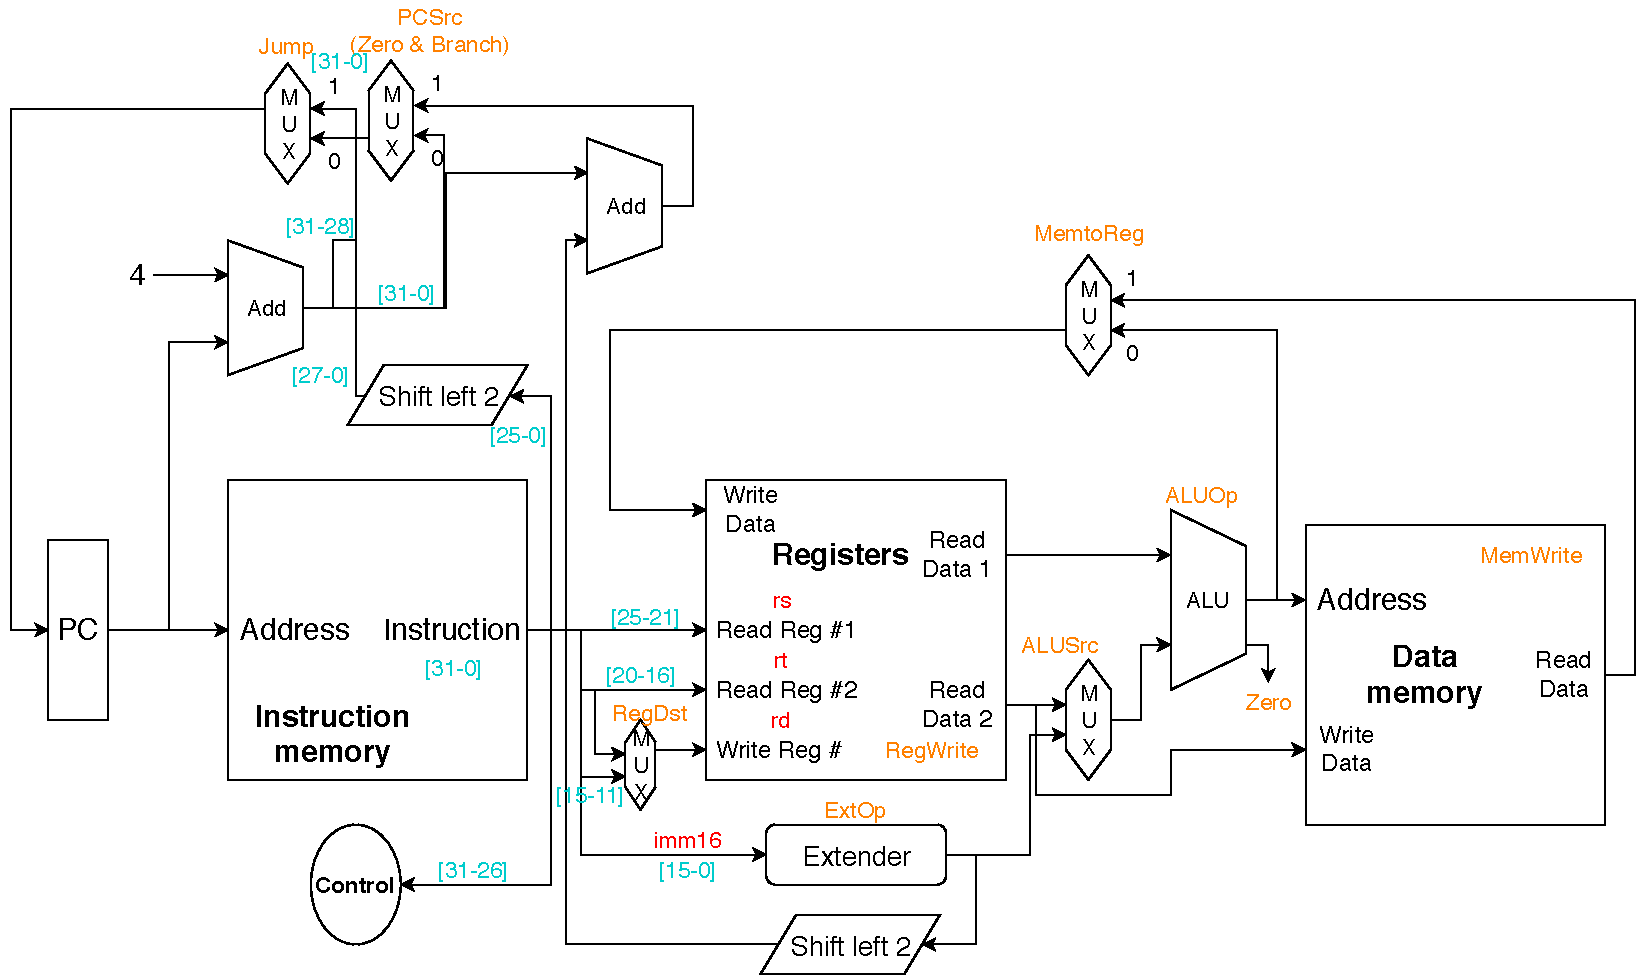
\includegraphics[width=\linewidth]{fig/Datapath_All.pdf}
\caption{MIPS基本数据通路}
\end{figure}
MIPS中三类基本指令:R-type、I-type、J-type\\
七条指令
\begin{enumerate}
	\item 加减 \verb'add/sub rd,rs,rt'
\begin{figure}[htbp]
\centering
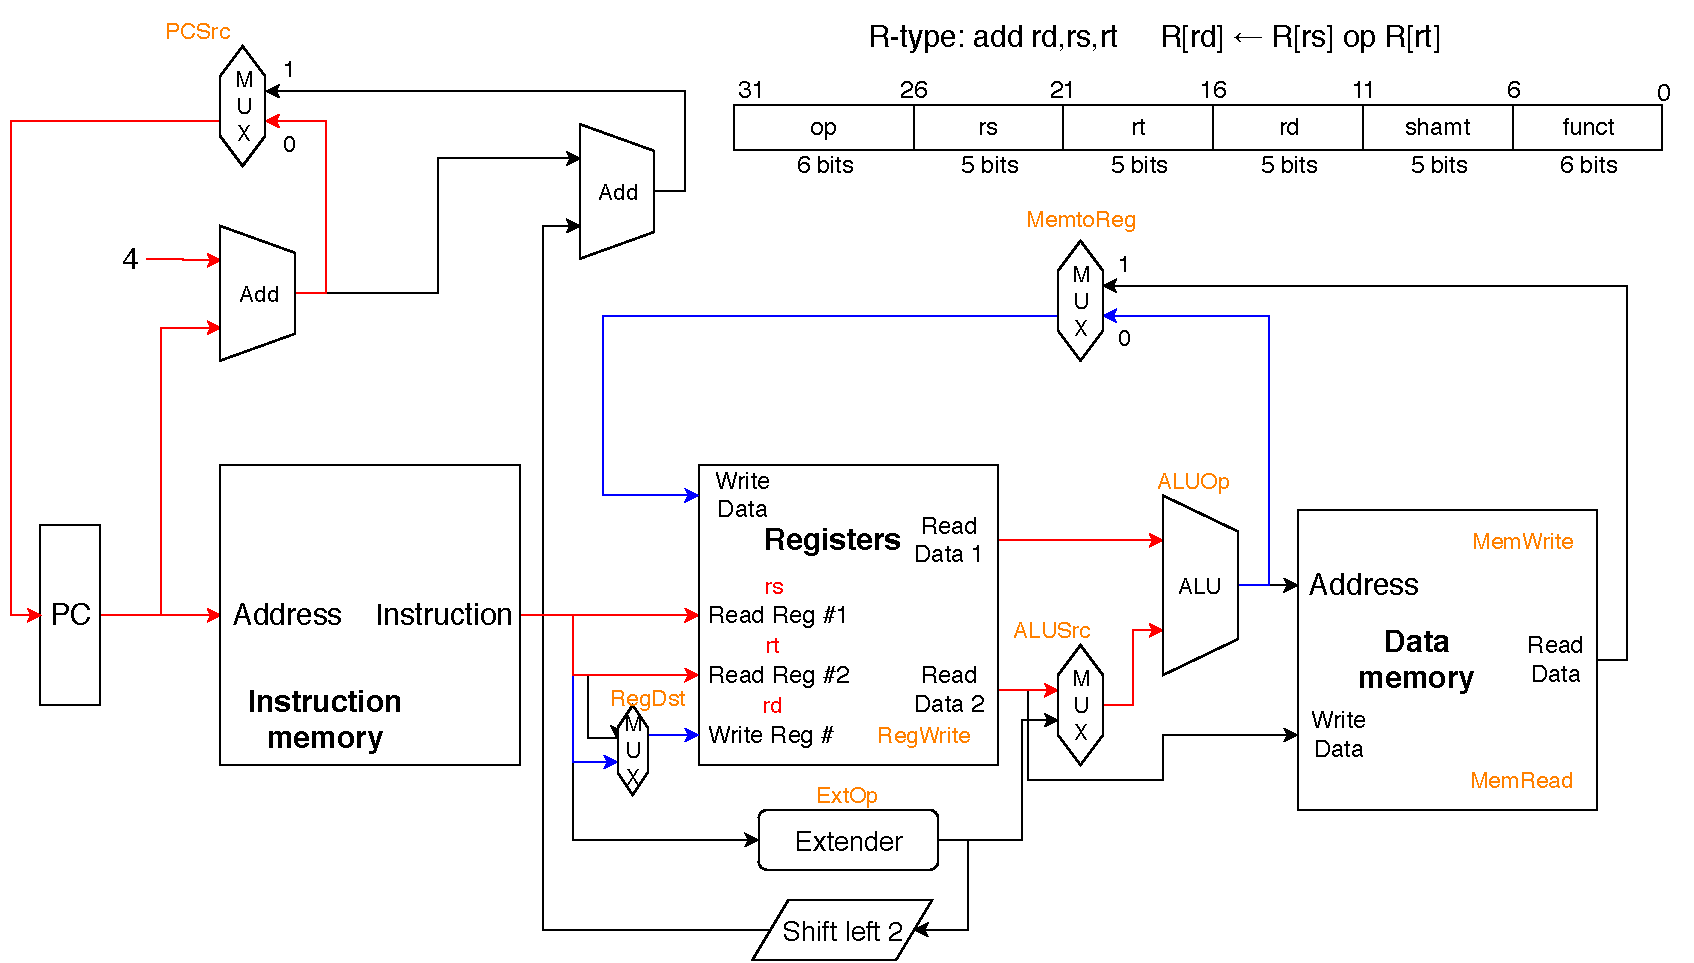
\includegraphics[width=\linewidth]{fig/Datapath_add.pdf}
\caption{add/sub通路}
\end{figure}
	\item 或立即数 \verb'ori rt,rs,imm16':零扩展
\begin{figure}[htbp]
\centering
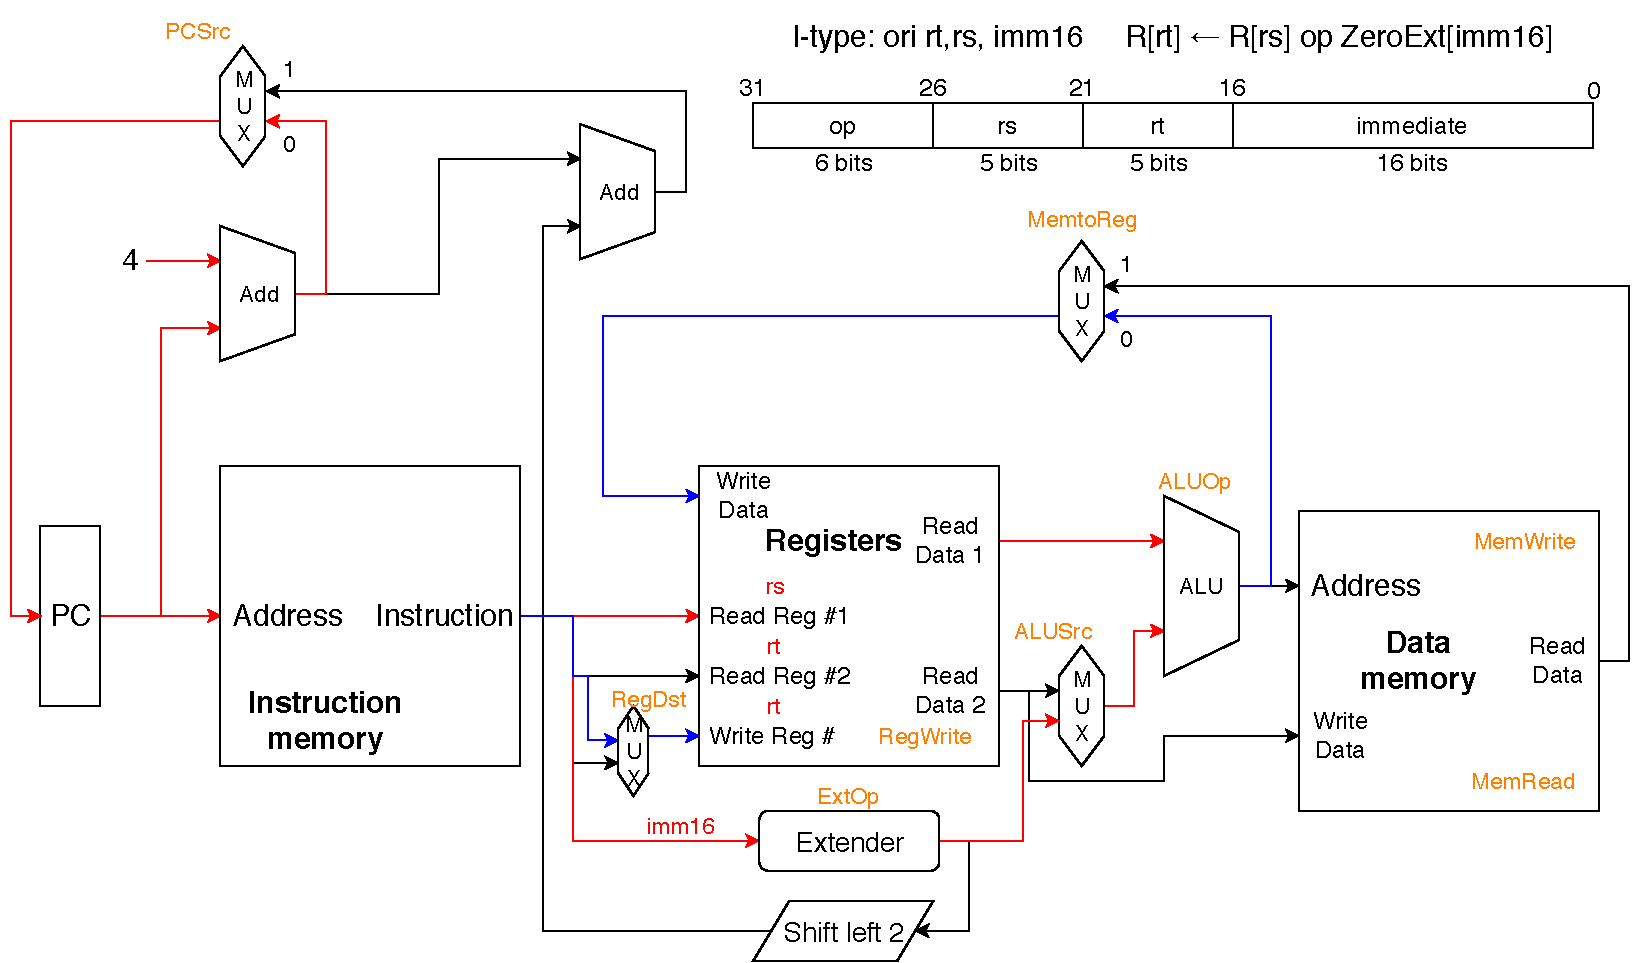
\includegraphics[width=\linewidth]{fig/Datapath_ori.pdf}
\caption{ori通路}
\end{figure}
	立即数需要零扩展(ZeroExt)为32位
	\item 存 \verb'lw rt,rs,imm16':符号扩展
\begin{figure}[htbp]
\centering
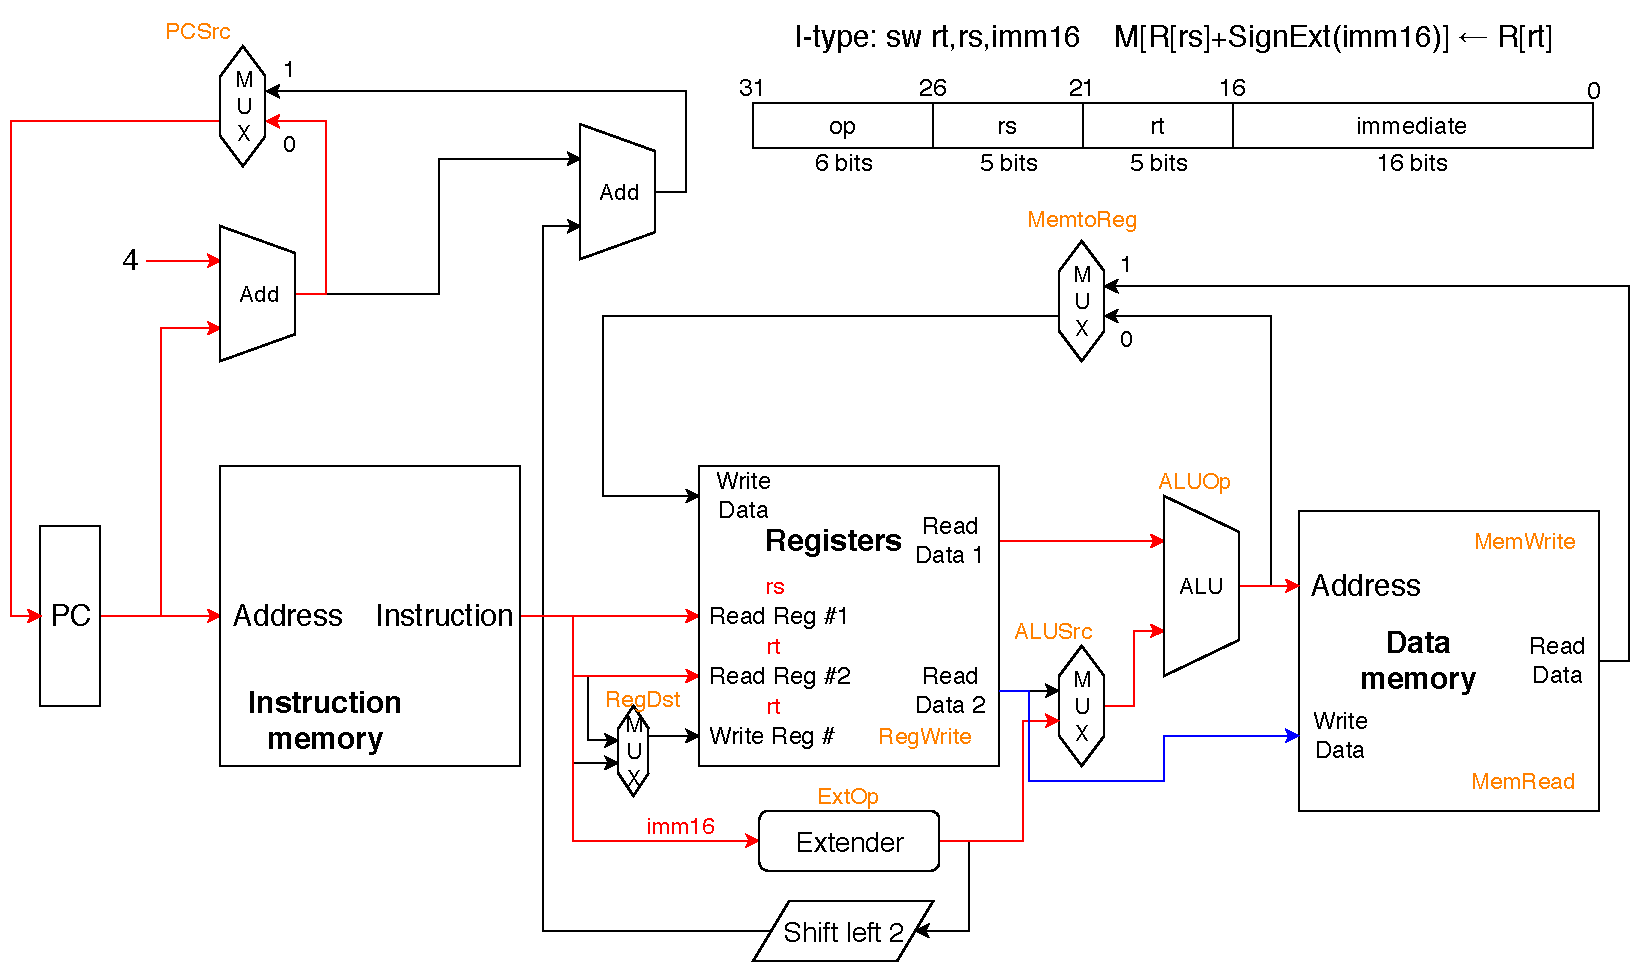
\includegraphics[width=\linewidth]{fig/Datapath_sw.pdf}
\caption{sw通路}
\end{figure}
	\item 取 \verb'sw rt,rs,imm16':符号扩展
\begin{figure}[htbp]
\centering
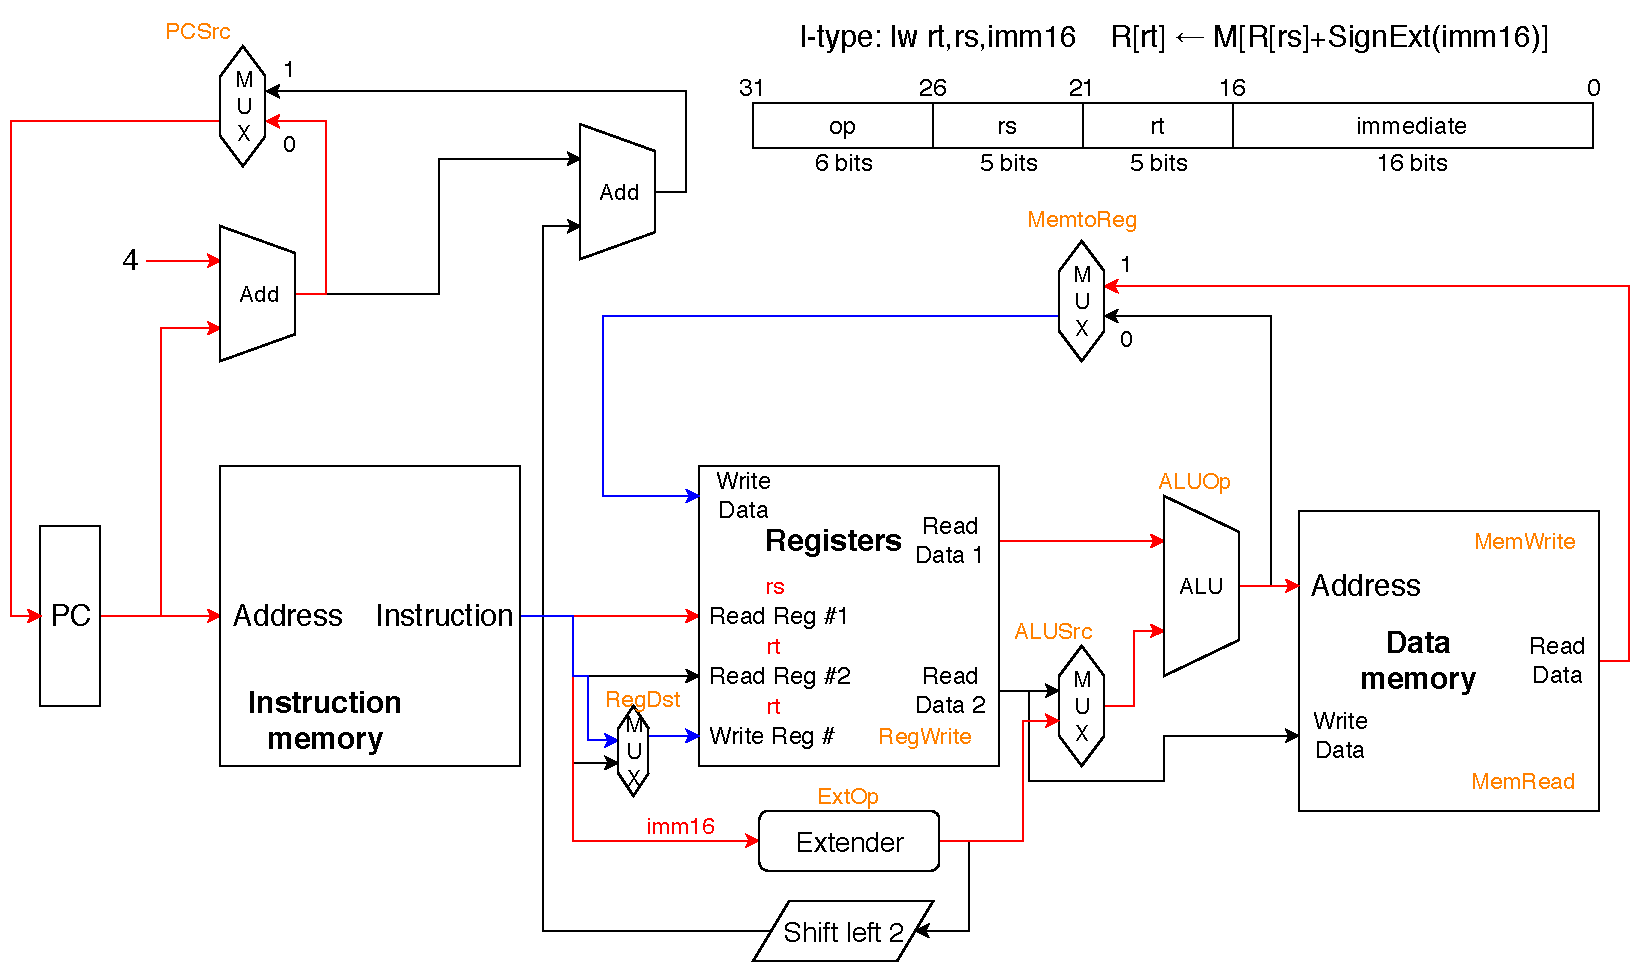
\includegraphics[width=\linewidth]{fig/Datapath_lw.pdf}
\caption{lw通路}
\end{figure}
	\item 分支 \verb'beq rs,rt,imm16':PC只需30位,因每次加4
\begin{figure}[htbp]
\centering
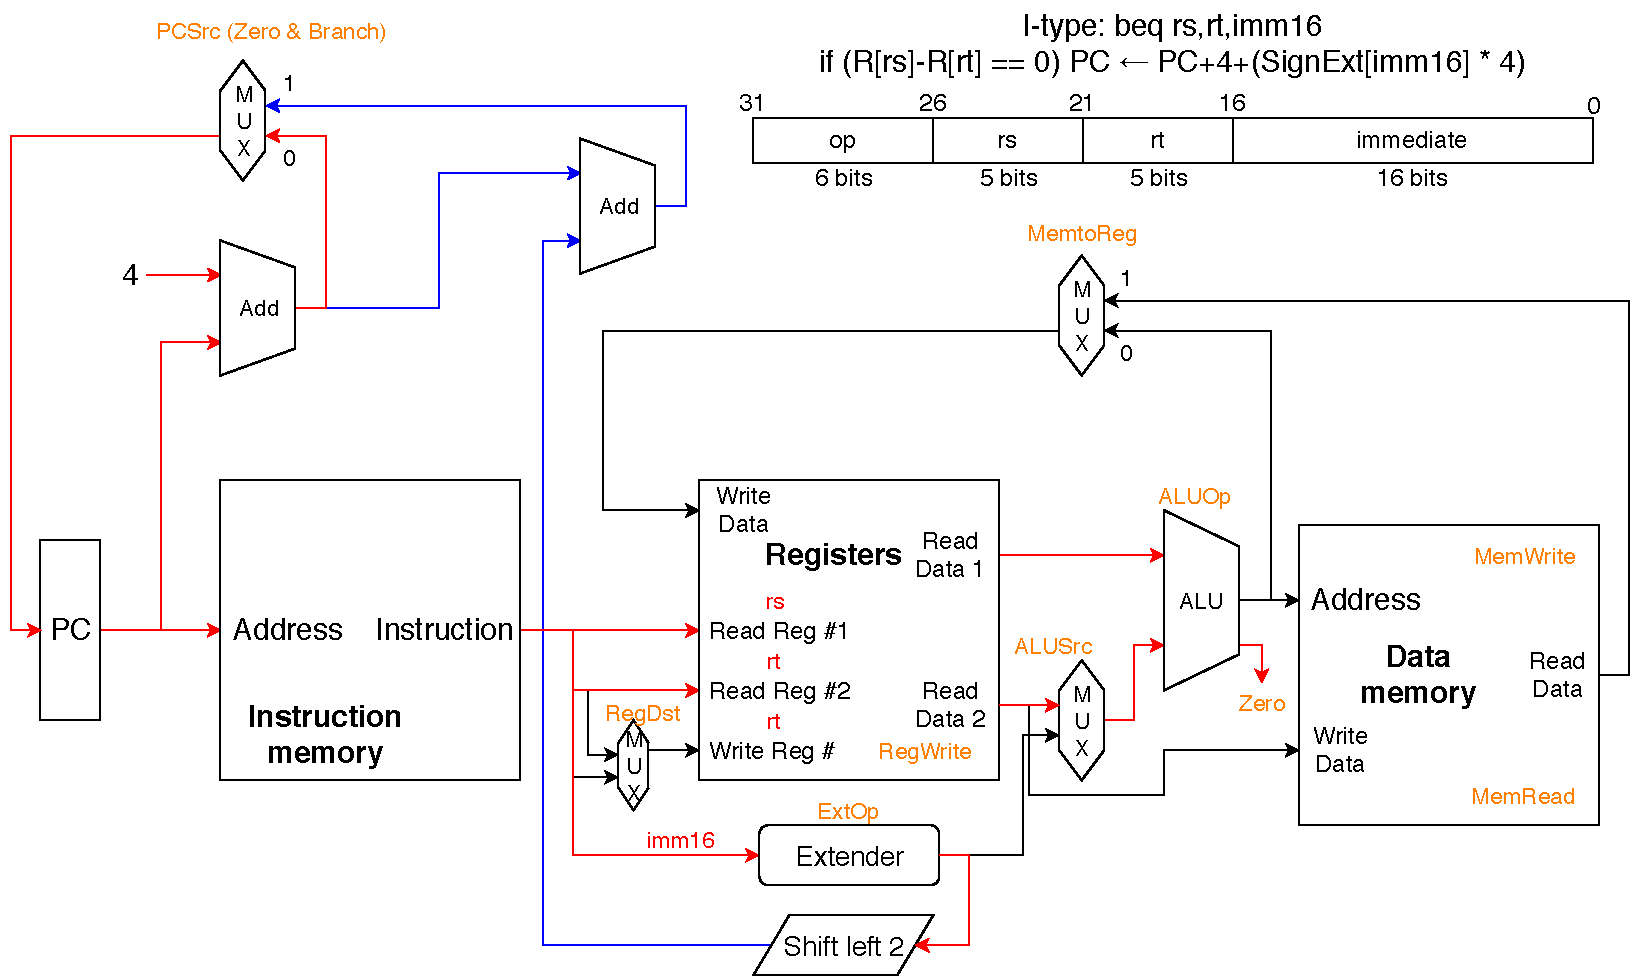
\includegraphics[width=\linewidth]{fig/Datapath_beq.pdf}
\caption{beq通路}
\end{figure}
	\item 跳转 \verb'j target':PC+4的高四位串接26位立即数然后左移2位
\begin{figure}[htbp]
\centering
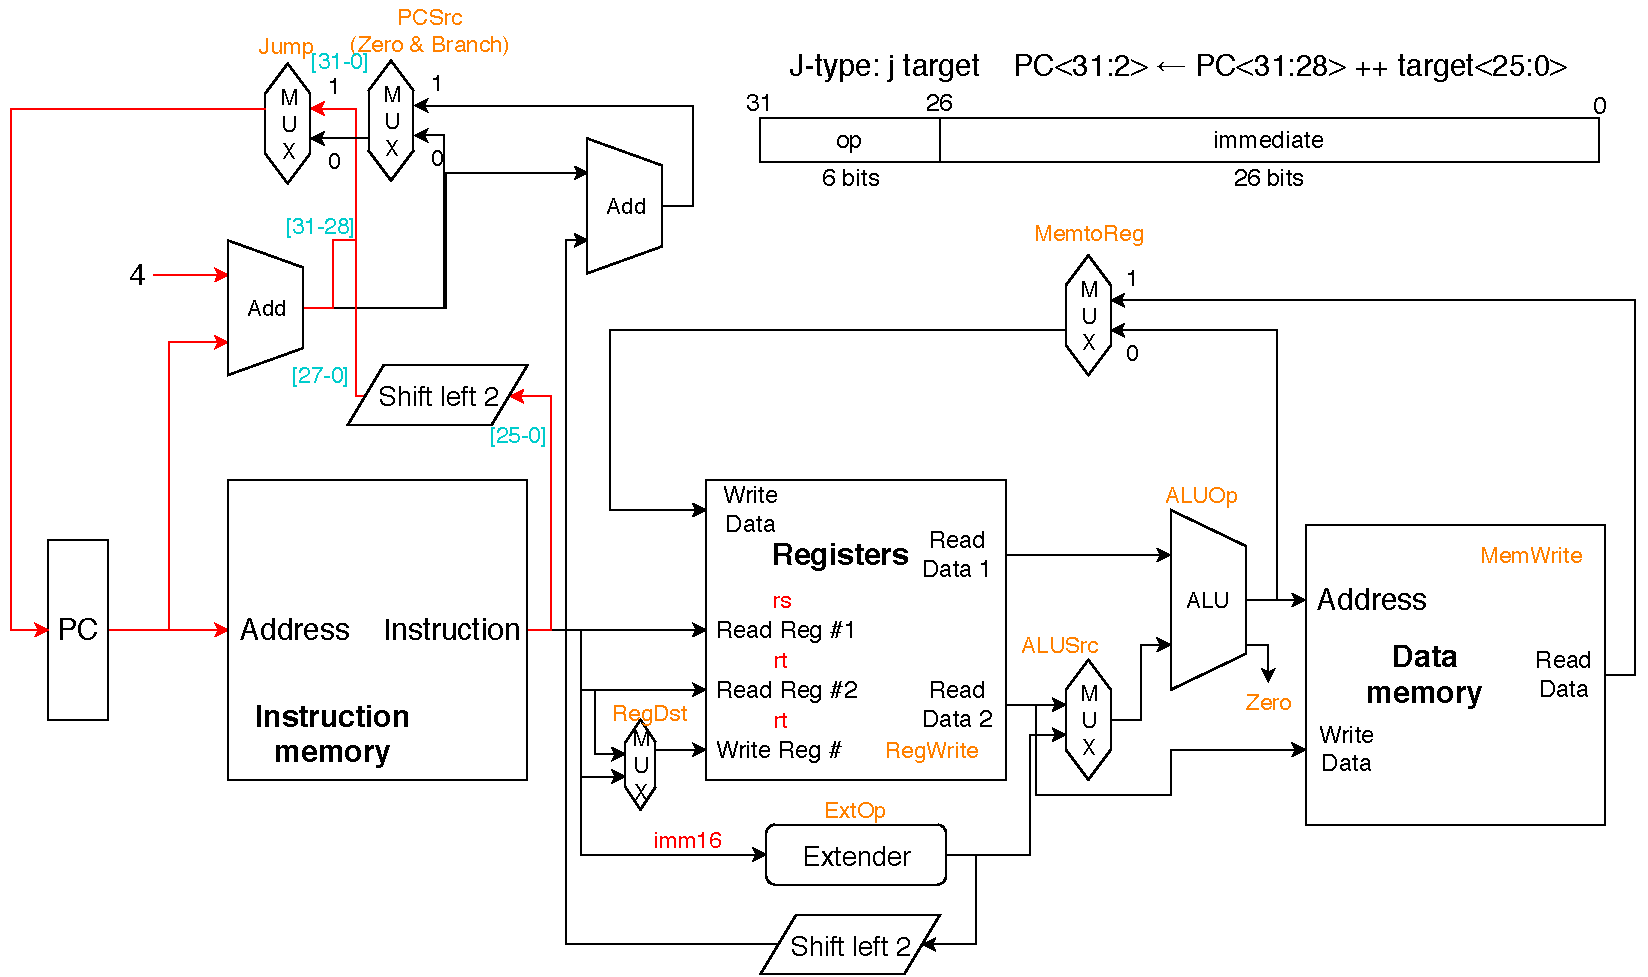
\includegraphics[width=\linewidth]{fig/Datapath_jump.pdf}
\caption{jump通路}
\end{figure}
\end{enumerate}

\subsection{多周期}
五个阶段:取指(IF)、译码(ID)、执行(EXE)、访存(MEM)、写回(WB)\\
\begin{itemize}
	\item 每个周期都在下个时钟到来时结束(此时存储元件被更新)
	\item 取指结束时PC+4开始写入PC,下个周期时,PC已被更新,置IRWr=0
	\item ALU空闲可用来投机计算转移地址
\end{itemize}
\begin{itemize}
	\item 有限状态机:通过组合逻辑硬连线(PLA)实现\\
	下一状态时当前状态和操作码的函数
	\item 微程序:用ROM存放微程序实现
\end{itemize}
\begin{figure}[htbp]
\centering
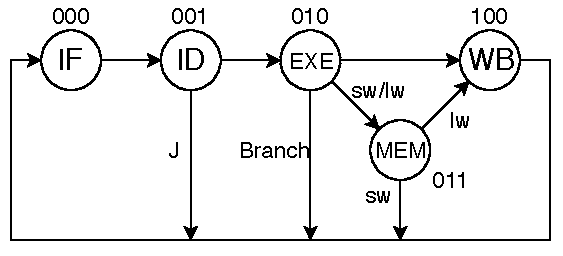
\includegraphics[width=0.5\linewidth]{fig/Datapath-Multi-cycle.pdf}
\caption{多周期CPU状态转移表}
\end{figure}
实际机器的寄存器组和存储器情况:
\begin{itemize}
	\item 寄存器有时钟输入,存储器可能无时钟输入
	\item 写操作不是由时钟边缘触发,而是一个组合电路:Din稳定,写使能为1,经过Write Access时间,才进行写入;会存在竞争问题
\end{itemize}

\subsection{流水线}
\subsubsection{概述}
提升工作主频:\\
减少每个流水级执行时间$\to$减少每个流水级的任务量$\to$任务再分解$\to$增加流水线级数\\
副作用:
\begin{itemize}
	\item 寄存器开销(overhead):收益下降
	\item 非均匀延迟(Nonuniform delays):吞吐率受限于最慢栈的时间,但很难将ALU和存储器划分成更小的栈
\end{itemize}
单个任务执行时间没有缩短,但是总的吞吐率增加了\\
时钟周期等于最长阶段花费时间$t$,N条指令执行时间$(5+N-1)\times t$\\
利于流水线执行的指令集
\begin{itemize}
	\item 指令长度一致:简化取指和指令译码
	\item 指令格式少,且源寄存器位置相同:利于在指令未知时预取操作数
	\item 只有load/store指令才能访问存储器,利于减少操作步骤,规整流水线
	\item 数据和指令在内存中\textbf{对齐}存放,利于减少访存次数和流水线规整
\end{itemize}

\subsubsection{冒险(Harzard)}
\begin{itemize}
	\item 结构冒险/资源冲突:一个功能部件同时被多条指令使用产生,如Load和R-type同时要写回
	\begin{itemize}
		\item 通过加空操作(NOP)延迟写操作(每条指令都有五个阶段)
		\item 设置多个部件(比如多个端口、寄存器读写口分开),避免冲突
	\end{itemize}
	\item 控制冒险/分支冒险/转移冒险:在jump/beq之前已有几条指令被取出
	\begin{itemize}
		\item 阻塞、NOP
		\item 分支预测
		\begin{itemize}
			\item 静态:总是预测条件不满足,或加启发式规则
			\item 动态:根据历史情况(Branch History Table, BHT)进行调整(微型强化学习)
		\end{itemize}
		\item 指令静态调度:编译优化指令顺序,实现分支延迟
	\end{itemize}
	\item 数据冒险/数据相关:写后读
	\begin{itemize}
		\item 转发(forwarding/bypassing):将数据从流水段寄存器中直接渠道ALU的输入端,如果在Data Memory读出则无法转发(Load-use数据冒险)
		\item 阻塞(stall):插入Bubble或插入NOP
		\item 静态指令调度:编译优化指令顺序,拉大具有数据冒险指令的距离,减少流水线可能产生的停顿(可以解决load-use);也即先把后面无关的操作调到前面来执行;或者说利用闲置资源先干后面的事情(乱序执行)% 只有在半并行(流水线)才会出现?
		\begin{figure}[htbp]
		\centering
		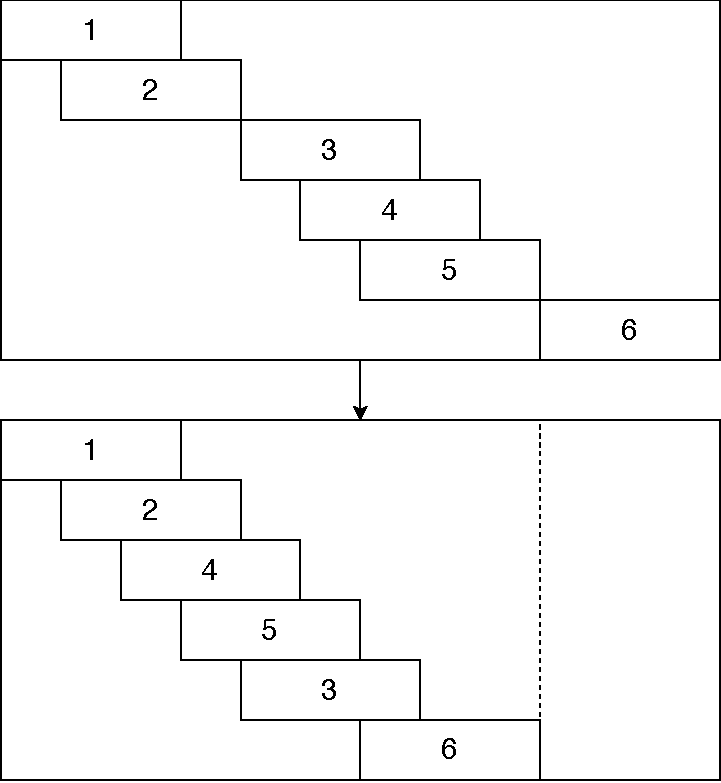
\includegraphics[width=0.3\linewidth]{fig/schedule.pdf}
		\caption{编译器调度}
		\end{figure}
	\end{itemize}
\end{itemize}

\subsubsection{指令级并行}
指令之间的相关性
\begin{itemize}
	\item 结构相关:同时存取相同寄存器或存储器
	\item 数据相关:RAW、WAR、WAW(注意中英文顺序区别)
	\item 控制相关
\end{itemize}
指令级并行(ILP)技术
\begin{itemize}
	\item 静态多发射:在执行前,由编译器帮助封装多条指令并处理冒险
	\begin{itemize}
		\item 发射包:可以在给定时钟周期内发射多条指令
		\item 发射槽:在给定时钟周期内能够发射指令的位置
		\item 超长指令字(VLIW):一类可以同时启动多个操作的指令集,一条指令来实现多个操作的并行执行
	\end{itemize}
	\item 动态多发射:在运行时,由处理器发射多条指令并处理冒险
	\begin{itemize}
		\item 超标量(superscalar):一种高级流水线技术,可以使每个周期处理器能执行的指令数超过一条\\
	试图在一个周期取出多条指令并行执行,通过在处理器中内置多条流水线来同时执行多个处理。本质是以空间换取时间,在不同流水线中不相关地执行多条指令。允许指令以不同于原程序顺序的次序执行
		\item 动态流水线调度:对指令进行重新排序以避免阻塞的硬件支持
	\end{itemize}
\end{itemize}
线程级并行(TLP)技术
\begin{itemize}
	\item 对于MIMD(多指令流多数据流),每个处理器执行自己的指令流
	\item 为了加大程序执行的并行力度,将程序划分为多个单一控制的执行流,每个执行流称之为一个线程。同一个进程中的不同线程共享数据空间,拥有自己的执行堆栈和程序计数器
	\item 提高系统整体的吞吐量
\end{itemize}
主要技术
\begin{itemize}
	\item 超线程(Hyper-Threading)技术
	\begin{itemize}
		\item Intel Xeon(2002)
		\item 允许物理上单个处理器采用共享执行资源的方法同时执行两个或更多的分离代码流(线程), 又称\textbf{软件多线程}
		\item 把单物理处理器模拟成2个或多个逻辑处理器,每个逻辑处理器都有独立的IA-32架构,即拥有自己的通用寄存器、段寄存器、控制寄存器、调试寄存器等
		\item 减少CPU的闲置时间,提高系统的资源利用率
		\item 逻辑处理器共享的资源包括执行引擎和系统总线接口
		\item 举例:两个线程整型\&浮点、运算\&I/O
	\end{itemize}
	\item 多核(Multi-Core)技术---空间并行
	\begin{itemize}
		\item Intel Core (2006)
		\item 通过在一个物理封装中集成多个分离的完整执行核来提供\textbf{硬件多线程}能力
		\item 每个完整的执行核拥有独立的指令集、执行单元,即不仅有自己的AS,还拥有自己的执行引擎,总线接口与L2 Cache等
		\item 本质是硬件的冗余,让不同处理器并发执行不同任务
		\item 效率与性能提升要比HT技术高得多
	\end{itemize}
\end{itemize}

\subsection{异常处理}
\begin{itemize}
	\item 内部异常(Exception):CPU发生的意外事件或特殊事件
	\begin{itemize}
		\item 硬故障中断:电源掉电、硬件线路故障等;机器将\textbf{终止},调出中断程序重启操作系统
		\item 程序性中断:执行某条指令时发生的异常
		\begin{itemize}
			\item 故障:执行指令引起的异常,如溢出、缺页、访问超时
			\item 自陷:预先安排的事件,如单步跟踪、系统调用等(自愿中断),处理完回到下条指令!
		\end{itemize}
	\end{itemize}
	\item 外部中断:CPU外发生的特殊事件,外界发送中断请求信号,如打印机缺纸、外设准备好、DMA传输结束等
\end{itemize}
检测到异常时,处理器需进行以下操作
\begin{itemize}
	\item 关中断:使处理器处于禁止中断状态
	\item 保护断点和程序状态:堆栈或特定寄存器
	\item 识别异常事件
	\begin{itemize}
		\item 软件识别:非向量中断(MIPS)\\
		EPC存放断点(异常处理后返回到的指令地址),总是存优先级最高的一个\\
		设置异常状态寄存器(Cause),操作系统用一个异常处理程序,按优先级顺序查询异常状态寄存器,识别出异常事件,转入相应的中断服务程序执行
		\item 硬件识别:向量中断(80x86)\\
		用专门的硬件查询电路按优先级顺序识别异常,得到“中断类型号”,到中断向量表中读取对应的中断服务程序的入口地址\\
		中断向量地址=中断类型号$\times$4
	\end{itemize}
\end{itemize}

\subsection{控制器}
现在常用折中方案:简单指令用硬连线,复杂指令用微控制
\subsubsection{硬连线控制器}
组合逻辑/有限状态机
\begin{itemize}
	\item 程序计数器PC
	\item 指令寄存器IR
	\item 节拍发生器Timing:有限状态机,确定指令执行顺序
	\item 控制信号产生电路CU
\end{itemize}

\subsubsection{微程序控制器}
\begin{center}
\begin{tikzcd}
\text{微程序(固件firmware)}\arrow{d}& \\
\text{微指令(一个状态)}\arrow{d} & \\
\text{微命令(控制信号)}\arrow{r} & \text{微操作(执行部件)}
\end{tikzcd}
\end{center}
微程序设计
\begin{itemize}
	\item 将传统的程序设计方法运用到控制器的逻辑设计中
	\item 用规整的存储逻辑代替不规则的硬接线逻辑来实现计算机控制器功能的技术
\end{itemize}
Wilkes模型(1951):输入指令寄存器IR中的操作码和机器状态标志;输出微操作控制信号\\
控制器处理一条指令的工作过程,就是启动这条指令在控制存储器中所对应的微程序,一条一条地顺序执行微指令的过程\\
微程序控制器工作过程
\begin{enumerate}
	\item IR中操作码经微程序顺序控制逻辑$\mu$C变换为该条指令微程序入口的微地址码
	\item 访问地址部件FCMAR选择微地址码,作为当前控制存储器的访问地址
	\item 根据地址从控制存储器读出一条微指令存入微指令寄存器中,其控制信号字段表示了当前运算器、存储器、控制器及FCMAR所需要执行的所有微操作
	\item 重复(2)、 (3),用微指令寄存器中地址码作为当前微地址码,直到一条指令对应的微程序执行完毕;接着执行一段微程序取下一条指令存放在IR中,然后返回(1)
\end{enumerate}
\begin{itemize}
	\item 程序计数器PC
	\item 指令寄存器IR
	\item 微指令下地址形成部件
	\item 控制存储器(只读,存放微程序)和微指令存储器
\end{itemize}
微指令格式:$\mu$OP、$\mu$Add(下条微指令地址)、常数(可选)\\
微指令编码方式:
\begin{itemize}
	\item 水平型微指令(面向控制逻辑):相容微命令尽量多安排在一条微指令中,最大限度并行
	\begin{itemize}
		\item 直接控制编码:不需译码,每个微命令用一位信息表示,易并行,但编码空间利用率低(即有多少个控制信号就多少位)
		\item 字段直接编码(显式编码):将微操作划分为若干小字段,每个字段单独编码,需译码
		\begin{itemize}
			\item 相容微操作:可同时进行,划分在不同字段
			\item 互斥微操作:不能同时进行,划分在同一字段
		\end{itemize}
		\item 字段间接编码(隐式编码):某些参与编码的微命令不能由一个控制字段直接定义,需要两个或两个以上的控制字段来定义
	\end{itemize}
	\item 垂直型微指令(面向算法):采用短格式,一条微指令只能控制一个微操作,速度慢
	\begin{itemize}
		\item 最短编码法:将所有微命令统一编码每条微指令只包含一个微命令,每次只产生一个微操作,通过译码器产生微操作控制信号;微程序长,大量译码电路,速度慢
	\end{itemize}
\end{itemize}
微指令地址产生方法:
\begin{itemize}
	\item 顺序转移(计数器)法:下条微指令地址隐含在微程序计数器$\mu$PC中
	\item 断定(下址字段)法: 当前微指令中显式指定下条微指令地址
\end{itemize}
% !TEX root = main.tex

\section{存储器的层次结构}
\subsection{概述}
存储器按照存储方式可分为以下几种:
\begin{enumerate}
	\item 随机访问存储器(RAM)\\
	存储器任意单元可随时访问且访问所需时间相同
	\begin{itemize}
		\item 静态(SRAM):cache\\
		\textbf{触发器}(寄存器也是);只要加电源,信息就能一直保持;集成度低,引脚多,速度快\\
		一般由以下几个部分组成:
		\begin{itemize}
			\item 存储阵列(存储体)
			\item 译码器电路
			\item 控制电路:$\overline{CE}$(Chip Enable), $\overline{WE}$(Write Enable), $\overline{OE}$(Output Enable)(后两个通常可合并)
			\item 数据缓冲电路
		\end{itemize}
		\item 动态(DRAM):主存\\
		\textbf{电容};每隔一段时间必须刷新;现在一般用DDR3 SDRAM(Double Data-Rate Synchronous)\\
		\begin{itemize}
			\item 分散式/异步刷新:在最大刷新间隔前将所有行刷新一遍
			\item 集中刷新
			\item 透明式刷新:每访存一次刷新一次
		\end{itemize}
	\end{itemize}
	\item 只读存储器(ROM):BIOS(Basic Input Output System)\\
	正常工作时只读,能随机读出,不能随机写入
	\begin{itemize}
		\item MROM:掩模式,只读
		\item PROM:一次性编程
		\item EPROM/EEPROM:多次改写,后者为电可擦除可编程存储器
	\end{itemize}
	\item 相联存储器(Content Addressed Memory, CAM):\textbf{快表(TLB)}\\
	按\textbf{内容}检索到存储位置进行读写
	\item 直接存取存储器(DAS):磁盘\\
	可以直接定位到要读写的数据块,存取时间的长短与数据所在位置有关
	\item 顺序存储器(SAS):磁带、电荷耦合器件CCD、VCD\\
	数据按顺序从存储载体的始端读出或写入,存取时间的长短与数据所在位置有关
\end{enumerate}
基本术语:
\begin{itemize}
	\item 记忆单元/存储位元/位元(Cell):具有两种稳态的能够表示二进制数0和1的物理器件
	\item 存储单元/编址单位(Addressing Unit):存储器中具有\textbf{相同地址}的那些位构成一个存储单元,又称为一个编址单位
	\item 存储体/存储矩阵/存储阵列(Bank):所有存储单元构成一个存储阵列
\end{itemize}
\begin{center}
存储位元 $\to$ 存储单元 $\to$ 存储矩阵 $\to$ 存储芯片(译码、驱动、读/写电路) $\to$ 存储模块(内存条) $\to$ 存储器
\end{center}
按照信息的可保存性分为:
\begin{itemize}
	\item 断电后数据是否丢失
	\begin{itemize}
		\item 挥发性(volatile)/易失存储器:SRAM、DRAM
		\item 非挥发性/非易失存储器(NVM):ROM、磁盘、闪存
	\end{itemize}
	\item 读出后是否保存数据
	\begin{itemize}
		\item 破坏性存储器(读出原信息被破坏,需重写):DRAM
		\item 非破坏性存储器:SRAM
	\end{itemize}
\end{itemize}
地址译码两种方式
\begin{enumerate}
	\item 线选法(一位地址译码)\\
	SRAM,只在单方向译码,同时读出一条字线上的所有位,$k$位地址对应$2^k$地址驱动线
	\item 位片式(二维双译码)\\
	$k$位地址对应$2^\frac{k}{2}+2^\frac{k}{2}$条地址驱动线\\
	若行列地址线复用,则可表示$2^{2k}$个地址
\end{enumerate}
\begin{example}
某一SRAM芯片,容量为1024$\times$8位,除电源和接地端外,该芯片数据与地址引脚的最小数目为?
\end{example}
\begin{analysis}
$1024B=2^{10}B$,故需10条地址线,8位则8条数据线,外加1条片选信号和1条读写控制线,共20条
\end{analysis}
\begin{figure}[H]
\centering
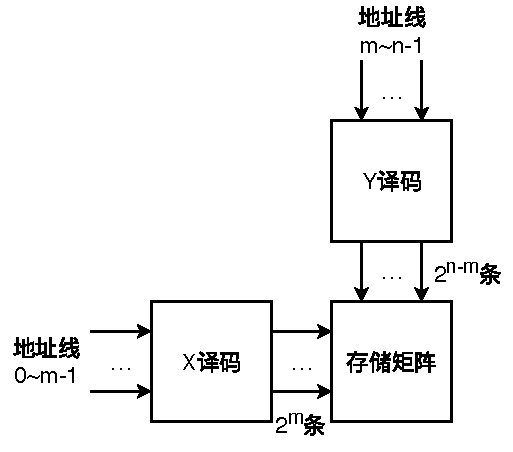
\includegraphics[width=0.4\linewidth]{fig/Memory-Double_Decode.pdf}
\end{figure}
存储器读写的时序:横线在中间为高阻,斜线为任意值,空白为有效
\begin{itemize}
	\item SRAM:行列地址同时送\\
	地址有效$\to$片选有效$\to$数据有效$\to$片选无效$\to$地址无效
	\begin{figure}[H]
	\centering
	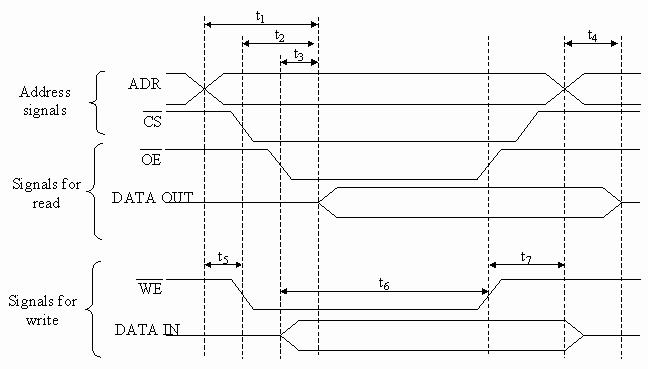
\includegraphics[width=0.4\linewidth]{fig/sram_cycle.png}
	\end{figure}
	\item DRAM:地址复用\\
	行地址有效$\to$行地址选通$\to$列地址、数据有效$\to$列地址选通$\to$数据输入$\to$全部无效
\end{itemize}
\begin{itemize}
	\item 读出时间$T_r$:从发出地址读命令到将数据读出来所需时间
	\item 存取周期$T_s$:连续两次读出两个主存单元所需的最小时间间隔(如DRAM要重写再生),$T_s<T_r$
\end{itemize}
多个请求同时读写存储器
\begin{itemize}
	\item 双端口存储器(时间并行):同时读写不同存储单元没有问题
	\item 多模块交叉存储器(空间并行):每个体都有自己的MAR、MDR和读写电路,可独立并行工作
	\begin{itemize}
		\item 连续编址(高位交叉):用主存地址码高位区分体号,低位表示模块内地址;存储地址连续的数据落在同一存储体内,易发生访存冲突(同时访问一个存储体),并行可能性小
		\item 交叉编址(低位交叉):以存储体个数(质数)为模交叉编址,把连续几个地址保存到不同存储器中;CPU同时送出m个地址,高位作为存储器地址,低位负责选择数据;由存储器分时使用数据总线进行信息传递(流水线)
	\end{itemize}
\end{itemize}
主存空间的划分
\begin{enumerate}
	\item ROM区:存放系统程序、标准子程序
	\item RAM区:存放用户程序
\end{enumerate}
带宽/数据传输率:每秒从主存中读出的二进制数据的数量

\subsection{存储容量扩展}
多少K就要多少根地址线,比如64KiB=$2^16$B就需要$A_0\thicksim A_{15}$地址线
\par 地址线、片选信号$\overline{CS}$、读写信号$\overline{WE}$、电源线、地线
\subsubsection{位扩展}
\begin{itemize}
	\item 存储芯片($mk\times n$位/片)构成存储器($mk\times N$位),需要$\lceil N/n\rceil$片
	\item 字数不变(存储单元个数不变),位数扩展(字长加长)
	\item 地址线及读写控制线相连接(同时读入),数据线单独引出,不需外部译码器/片选信号
\end{itemize}
\begin{figure}[H]
\centering
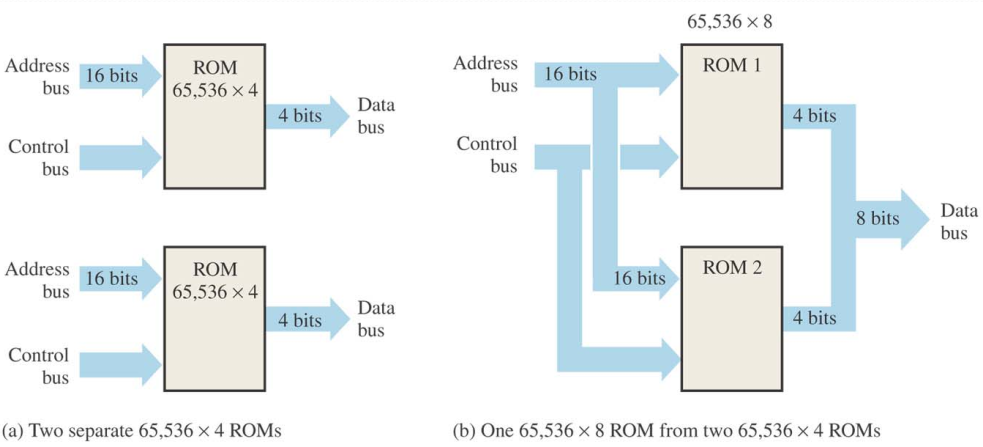
\includegraphics[width=0.6\linewidth]{fig/word-length.PNG}
\end{figure}

\subsubsection{字扩展}
\begin{itemize}
	\item 存储芯片($mk\times n$位/片)构成存储器($Mk\times n$位),需要$\lceil M/m\rceil$片
	\item 位数不变(字长不变),扩充容量(存储单元个数增加)
	\item 地址线、读写控制线对应相接,但需要加片选信号(与外部译码器相连)
\end{itemize}
\begin{figure}[H]
\centering
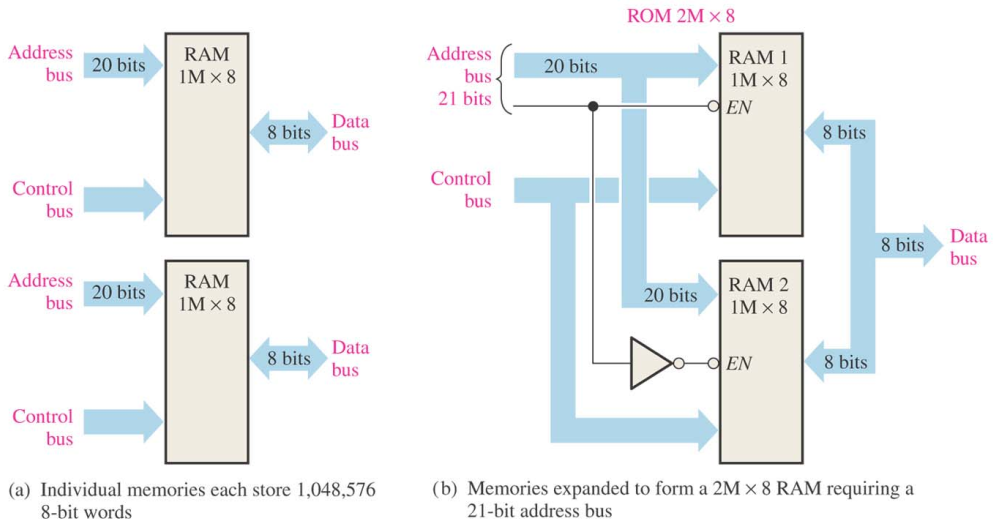
\includegraphics[width=0.6\linewidth]{fig/word-capacity.PNG}
\end{figure}

\subsubsection{字位扩展}
\begin{example}
用1K$\times$4b的DRAM芯片(64$\times$64结构)构成16K$\times$16b的存储器
\end{example}
\begin{analysis}
\begin{enumerate}
	\item 所需芯片数目:32KB/0.5KB=64
	\item 位扩展16/4=4个,字扩展16/1=16组
	\item 总共需14条地址线,因16K=$2^{14}$
	\item 其中字扩展需要4个片选信号$16=2^4$,4条线
	\item 片内寻址10条地址线
	\item 刷新周期$64T_{refresh}<T_{max}$
\end{enumerate}
\end{analysis}

\subsection{存储器与CPU的连接}
通信方式
\begin{itemize}
	\item 异步(需握手)
	\item 同步:CPU和主存由统一时钟信号控制,无需应答
\end{itemize}
主存空间的划分
\begin{itemize}
	\item ROM存放系统程序、标准子程序
	\item RAM存放用户程序
\end{itemize}
注意74LS138还有三个使能端$G_1,\overline{G_{2A}},\overline{G_{2B}}$


\subsection{Cache概述}
\subsubsection{计算机存储层次结构}
大容量、高速度、低成本\\
多级系统的存储容量即为最底层的存储容量,因为是包含关系\\
CPU与cache之间以字为单位传送,cache与主存之间以块为单位传送\\
程序访问局部性
\begin{itemize}
	\item 时间(temporal)局部性:刚被访问过的存储单元很可能不久又被访问,如循环变量
	\item 空间(spatial)局部性:刚被访问过的存储单元的邻近单元很可能不久被访问,如数组顺序访问
\end{itemize}
cache对程序员是透明的,即程序员在编写程序时无需了解cache是否存在或如何设置

\subsubsection{命中与失效}
\begin{itemize}
	\item 命中(hit):要访问的信息在cache中
	\item 失效(miss):不在cache中
\end{itemize}
平均访问时间
\[\bar{T}=pT_h+(1-p)(T_h+T_m)=T_h+(1-p)T_m\]
影响因素
\begin{itemize}
	\item cache越大,失效率越低,但成本越高
	\item block越大,失效率越低;但block在cache中所占比例增加到一定程度,失效率会上升
	\item cache容量小时,映射方式有影响;容量大时,影响不大
\end{itemize}

\subsection{cache与主存的映射}
cache存放一个主存块的对应单位为行(line)或块(block)或槽(slock)或项(entry)\\
位宽即为cache一个块的大小,如传送单位为512B,则cache每个块大小为512B\\
增大块的大小,以利用空间局部性\\
频繁的cache替换称为cache抖动

\subsubsection{直接(direct)映射}
cache内存放的内容是主存的一个子集,因此给出一个主存地址,要在cache中找到这个地址,应该将这个32位地址全部用上。末几位用于确定在cache内存储的位置,高位(tag)则用来确定是否为该地址。
\begin{itemize}
	\item 注意区别块地址、字地址、字节地址等(一般按字节编址)
	\item 按字索引则后两位不需要
	\item 先计算出块地址(因而先模块内数目),再计算块内地址
	\item $0\thicksim n-1$块称为第0区/块群,$n\thicksim 2n-1$称为第1块群,以此类推
\end{itemize}

\subsubsection{全相联(full associative)映射}
比较地址要与所有单元比较,线路复杂,成本高

\subsubsection{组相联(set associative)映射}
直接模组的数目。
相联度高,缺失率低,但会增加命中时间
只要命中了tag则对应的主存块一定在cache里
\begin{figure}[H]
\centering
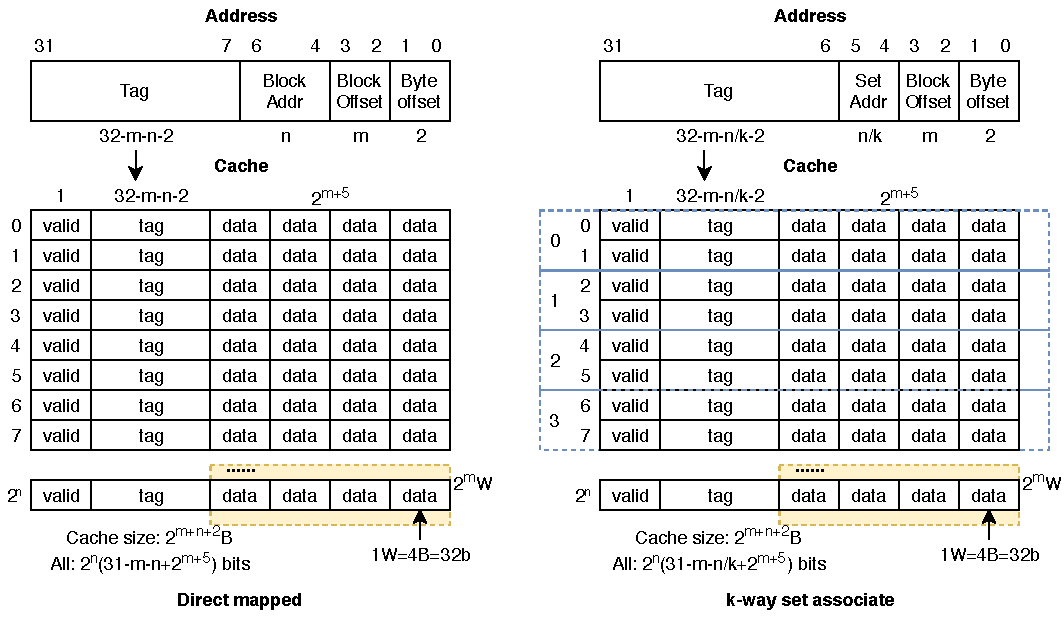
\includegraphics[width=0.8\linewidth]{fig/Cache-combine.pdf}
\end{figure}

\begin{example}
某一直接映射的cache容量为8K字,每块内有16个字,主存容量为512K字
\end{example}
\begin{analysis}
\begin{itemize}
	\item 主存有$512K=2^{19}$个字,$512K/16=2^{19}/2^4=2^{15}$个块,$512K/8K=2^6$个区
	\item cache有$8K=2^{13}$个字,$8K/16=2^{13}/2^4=2^9$个块
	\item 主存字地址19位,区号6位,区内块号15-6=9位,块内地址4位($16=2^4$)
	\item cache字地址13位,块号9位,块内4位
	\item 主存第$i$块位于第$\lfloor i/2^9\rfloor$个区,调入cache第$i\;\mod 2^9$块
\end{itemize}
\end{analysis}


\subsection{Cache替换算法}
\begin{itemize}
	\item FIFO
	\item Least Recently Used (LRU)比较好:给每一个cache行设定一个计数器,值越小越经常被使用;不被用则加1
	\item Random
\end{itemize}

\subsection{Cache一致性}
\begin{itemize}
	\item 写命中(hit)
	\begin{itemize}
		\item 写直达(write through):同时写cache和主存\\
		加入写缓冲(write buffer),先存入写缓冲,当写主存操作结束后再将写缓冲数据释放
		\item 写回(write back):只写cache不写主存,没有同步更新!\\
		每个cache行置一个脏位(dirty bit),若cache行中的主存块被修改,则置为1;只有当脏位为1的块从cache中替换出去时才将其写回主存
	\end{itemize}
	\item 写不命中(miss)
	\begin{itemize}
		\item 写分配(allocate-on-miss):更新主存块相应单元,再将该主存块装入cache(空间局部性)
		\item 写不分配(no-allocate-on-write):直接写主存,不放回
	\end{itemize}
\end{itemize}
通常写直达+写分配/写不分配,写回+写分配

\subsection{多级Cache}
一般L1 Cache为分立Cache(数据指令分开放),减少命中时间获得较短时钟周期\\
L2 Cache为联合Cache,降低缺失率以减少主存缺失损失\\
Intel Core i7采用三级Cache
\begin{center}
\begin{tabular}{|c|c|c|}\hline
L1 & L2 & L3\\\hline
32KB I/ 32 KB D & 256KB & 2MB/core\\\hline
4-way I/8-way D & 8-way & 16-way \\\hline
Pseudo-LRU & Pseudo-LRU & \begin{tabular}{l}Pseudo-LRU\\+ordered selection algorithm\end{tabular}\\\hline
\end{tabular}
\end{center}

\subsection{虚拟存储器}
产生原因:同时运行更多进程,内存需求增大
\begin{enumerate}
	\item 允许多个程序有效而安全地共享存储器,消除内存因小而有限的容量给程序设计造成的障碍
	\begin{itemize}
		\item 可以更有效功效处理器和主存
		\item 虚存实现程序地址空间道物理空间的转换,加强了各个程序地址空间之间的保护
	\end{itemize}
	\item 允许单用户程序大小超过主存容量,虚存自动管理主存和辅存组成的两级层次结构
\end{enumerate}
\subsubsection{概述}
Cache解决系统速度,虚存解决系统容量\\
Cache全硬件管理,而虚存由硬件和OS共同管理
\begin{itemize}
	\item 将内外存统一管理的存储管理机制,按需调页(demand paging)
	\item 虚存是主存和磁盘的抽象,OS使每个进程看到的存储空间都一致
	\item 虚存为每个进程提供一个假象,好像每个进程都独占主存,且主存空间极大
\end{itemize}
\par 分页(paging)基本思想
\begin{itemize}
	\item 将内存分为固定长且较小的存储块,每个进程也划分为固定长度的程序块
	\item 程序块(页/page)可装到存储器可用的存储块(页框/page frame)中
	\item 无需用连续页框来存放一个进程,只需将当前活跃页面调入主存
	\item 操作系统为每个程序/进程生成一个页表(page table)
	\item 通过页表实现逻辑地址到物理地址的转换(address mapping)
	\item 只有进程最后一个零头(内部碎片)不能使用,浪费小
\end{itemize}
逻辑地址与物理地址区别
\begin{itemize}
	\item 逻辑地址:程序中指令所用的地址
	\item 物理地址:存放指令或数据实际内存地址
\end{itemize}
段式虚拟存储器
\begin{itemize}
	\item 段是程序本身的属性,且可以有不同长度,可自由调度
	\item 段本身是程序的逻辑结构所决定的一些独立部分,所以分段对程序员是不透明的(而分页是透明的)
	\item 但因长度可变,分配主存空间不便,容易产生内存碎片
\end{itemize}
段页式虚拟存储器
\begin{itemize}
	\item 程序按模块分段,段内再分页,进入主存仍以\textbf{页}为基本单位
	\item 逻辑地址由段地址、页地址和页内偏移量三个字段构成
	\item 用段表和页表(每段一个)进行两级定位管理
	\item 根据段地址到段表中查阅与该段相应的页表指针,再转向页表,然后根据页地址从页表中查到该页在主存中的页框地址,由此访问到页内某数据
\end{itemize}

\subsubsection{组织方式}
页式虚拟存储器,存在主存中
\begin{itemize}
	\item 指令给出虚拟地址
	\item 每个页表记录对应的虚页情况
	\item valid为0说明缺页(page fault),代价读磁盘,软件处理:当前指令执行被阻塞,当前进程挂起;缺页处理结束后,回到原指令继续执行
	\item 当读写操作不符合access right时,发生保护违例
	\item CPU执行指令时,先由内存管理单元(MMU)将逻辑地址转为物理地址
	\item 页大小比cache的block大得多,全相联映射
	\item 写回策略
\end{itemize}
页表结构
\begin{itemize}
	\item 每个进程一个页表
	\item 页表项即为页表中的一项,即物理地址(页号+页内偏移)
	\item 页表项数由进程大小决定
	\item 页表在主存的首地址记录在页表基址寄存器中
\end{itemize}
页面大小不能太小,否则页面个数多,页表太大;也不能太大,一次装入页面时间太长
\begin{example}
某页式虚拟存储器,有32位虚拟地址,页大小为4KB,每个页表项占4B,则操作系统为进程分配的页表最大为多少?
\end{example}
\begin{analysis}
最大页表项数=最多页的数目=$2^{32}/2^{12}=2^{20}$\\
最大页表大小=页表项数$\times$每个页表项大小=$2^{20}\times 2^2B$=4MB
\end{analysis}
\begin{example}
虚拟地址16位,物理地址12位,页大小为128B,TLB采用四路组相联,共16个页表项
\end{example}
\begin{analysis}
页大小$2^7$B,故7位用来做页内偏移\\
四路组相联,16个页表项,即4个组,故2位组偏移(TLB索引)\\
其余6位为TLB标志位,即$15\thicksim 7$位都为虚拟页号\\
页内偏移不变,其余用来做物理页号
\end{analysis}

\subsubsection{快表(TLB)}
转换后备缓冲器(Translation-Lookaside Buffer),存在cache中\\
每次读写操作都至少带来两次存储器访问,一次访问页表,一次访问所需的数据或指令\\
使用cache来存储页表项,它包含了最近使用的那些页表项\\
不可能页表miss了,快表hit了,因为页表缺失,信息一定不在主存页不在cache
\begin{figure}[H]
\centering
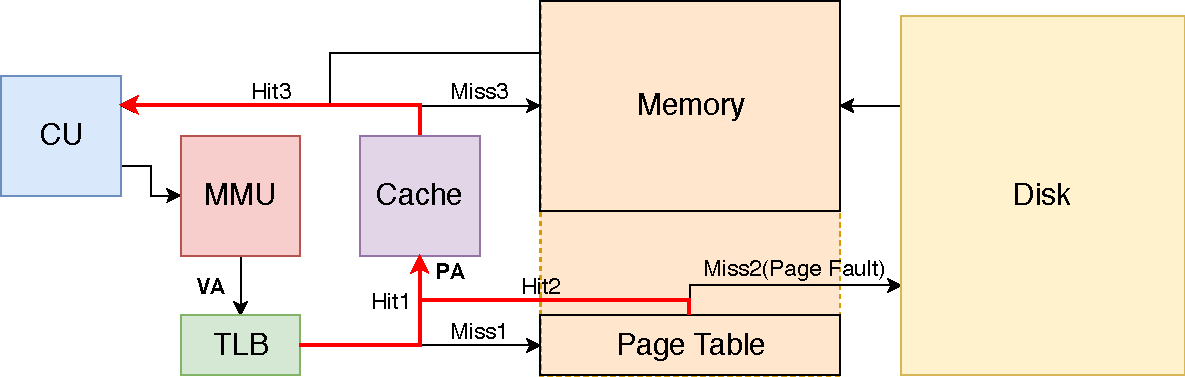
\includegraphics[width=0.8\linewidth]{fig/Cache-page.pdf}
\end{figure}
TLB指标
\begin{itemize}
	\item 多用全相联:命中率高
	\item 采用随机替换策略:降低替换算法开销
	\item 写回策略:减少访存次数
	\item 大小:$16\thicksim 512$项
	\item 块大小:$1\thicksim 2$项(每个表项$4\thicksim 8$B)
	\item 命中时间:$0.5\thicksim 1$个时钟周期
	\item 失靶损失:$10\thicksim 100$个时钟周期
	\item 命中率:$90\thicksim 99\%$
\end{itemize}
\begin{figure}[H]
\centering
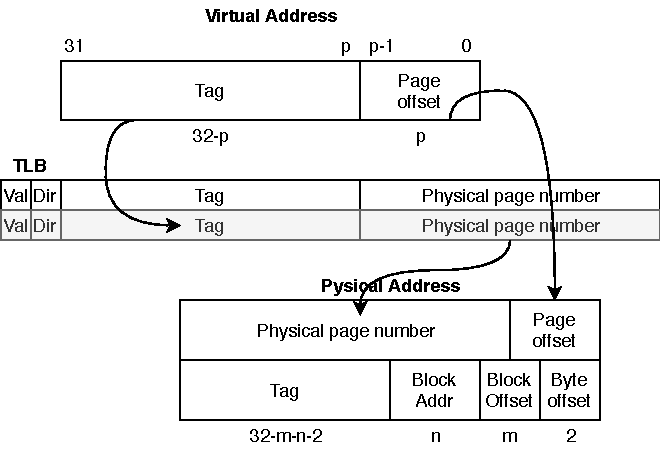
\includegraphics[width=0.6\linewidth]{fig/Cache-page_address.pdf}
\end{figure}

\subsubsection{存储保护}
\begin{itemize}
	\item 地址越界:转换到的物理地址不属于可访问范围
	\item 访问越权:访问操作所拥有的访问权限不符
\end{itemize}
通过程序重定位进行存储区域保护
\begin{itemize}
	\item 静态:在装入前将所有地址全部转为物理地址,通过给逻辑地址加界/基准地址实现
	\item 动态:由硬件地址转换机构实现
\end{itemize}

\subsection{并行主存系统}
\begin{itemize}
	\item 均匀存储访问模型(UMA, Uniform Memory Access):访问任何存储字时间相同
	\item 非均匀存储访问模型(NUMA):被共享的存储器在物理上分布于各个处理器
\end{itemize}
多处理器的cache一致性
\begin{itemize}
	\item 软件:编译使得共享数据只放在主存,不放入高速缓存
	\item 硬件:硬件协议维护,关键在于跟踪所有共享数据块的状态
	\begin{itemize}
		\item 侦听协议(snooping):侦听到主存中一个单元被修改则将自己cache中单元副本置为无效或更新
		\item 目录协议:在主存中设置一个目录表,记录共享数据的所有高速缓存行的位置和状态
	\end{itemize}
\end{itemize}
% !TEX root = main.tex

\section{输入输出系统}
\subsection{IO接口}
IO接口是主机与IO设备之间数据交换的界面,它屏蔽了IO设备的差异,提供了一致的访问界面
\par 功能如下
\begin{enumerate}
	\item 数据格式(串并)转换和电平变换
	\item 数据缓存(速度不匹配)
\end{enumerate}
IO端口:IO接口中的各类寄存器\\
一个IO接口可以有多个地址,因多个寄存器\\
IO指令实现的数据传送通常发生在通用寄存器和IO端口之间
寄存器编址
\begin{itemize}
	\item 统一编址,与主存统一编址,可以用访存指令去访问外设中的存储器
	\item 独立编址,对IO端口单独编号,需要专门的IO指令
\end{itemize}
% IO设备的连接 6.2
接口芯片有使能端CS
\begin{example}
CRT显示器分辨率为1027*768像素,像素的颜色数位65536色,则刷新存储器的容量至少是?
\end{example}
\begin{analysis}
颜色种数$65536=2^{16}$,即16位色,用2B表示\\
总共$1024*768*2B=1536KB$
\end{analysis}

\subsection{磁盘存储器}
磁盘组织:磁道、扇区(访问信息最小单位)、柱面\\
通常将同一文件存放在不同面的同一磁道上,以提高存取效率\\
道(track)密度:垂直于磁道方向上(半径方向)单位长度磁介质所容纳的磁道数\\
位(bit)密度:单位长度磁道上所能记录的二进制信息位数\\
面(surface)密度:单位面积上记录的二进制信息位数=道密度$\times$位密度\\
存取时间$t$=寻道时间$t_s$+旋转等待时间$t_w$+数据传输时间($t_{WR}$)\\
最大旋转延迟=1/磁盘转速*60s/1min\\
平均旋转延迟=最大旋转延迟/2(旋转半圈时间)\\
硬盘容量=柱面$\times$磁头数$\times$每磁道扇区数$\times$每扇区字节数\\
转速单位为rpm或r/min
\begin{example}
设磁盘平均寻道时间为10.5ms,磁盘的转速为3000转/分,每个扇区的字节数为512,每条磁道的容量为3072字节,则磁盘存储器读写一个扇区平均访问时间为?
\end{example}
\begin{analysis}
转速50转/分,则每转半圈为$t_w=0.01s$\\
数据传输时间(即扫过一个扇区所需时间,或扇区数据量/一s扫过的数据量)$t_{WR}=512B/(3072B\times 50)=3.33ms$\\
故$t=10.5ms+10ms+3.33ms=23.83ms$
\end{analysis}

\subsection{闪存存储器}
电可擦写、可编程只读存储器(EEPROM)
\begin{itemize}
	\item NOR:随机,可以直接按字节访问,主要用于存储程序代码(code)
	\item NAND:块级IO访问,主要用于存储数据(data)
\end{itemize}
读快、写慢(块擦)\\
通过损耗均衡(wear leveling)减少块的磨损\\
固态盘SSD即为闪存

\subsection{光存储器}
光存储器(Optical Disk Memory, ODM):采用激光手段对存储介质进行读写操作
\begin{itemize}
	\item 工作原理:将激光聚焦成极细光束在存储介质上存储信息,根据激光束和反射光的强弱不同,实现信息读写
	\item 优点:光盘记录密度高,单片存储容量大,非接触式读写,易于更换保管,对环境条件没有苛求
	\item 缺点:光盘机寻道时间长,可擦写性能不如磁盘快
\end{itemize}
按记录介质分类
\begin{itemize}
	\item 形变型光盘:不可逆,如CD-ROM、VCD、DVD-ROM
	\item 相变型光盘(Phase Change Disc, PCD):不可逆、可逆
	\item 磁光型光盘(Magneto Optical Disc, MDO):可多次读写
\end{itemize}
蓝光存储密度高

\subsection{RAID盘阵}
计算机系统总体性能的提高很不匹配:处理器和主存性能改进快,但辅存性能改进慢
\par 廉价磁盘冗余阵列(Redundant Array of Inexpensive Disks, RAID)
\begin{itemize}
	\item 多个廉价磁盘增加容量(类似多体交叉)
	\item 并行工作提高数据传输速度
	\item 冗余进行错误恢复,进而提高系统可靠性
\end{itemize}
\begin{enumerate}
	\item RAID0:条带化;存储容量、读写速度,但可靠性不够
	\item RAID1:镜像盘1+1冗余;有可靠性,但无存储容量、读写速度
	\item RAID2:条带化+海明校验码;冗余信息开销大,读性能高,写要同时写数据盘和校验盘,性能低
	\item RAID3:奇偶校验法生成单个冗余盘,条区增大为KB,提高吞吐率;适用于大量顺序数据访问的应用场合,如医学图像处理等;某个磁盘损坏时,可以通过其它磁盘重新生成;校验时,须将所有未写数据盘的原数据全部读出,再与写入盘的新数据异或形成新校验数据,并将其写入校验盘
	\item RAID4:独立存取技术, 使用更大条区,各个盘相互独立访问,并发I/O,共享的校验盘;适合于较小的数据访问,允许并发地发生多个独立访问;多个并发写时,唯一的共享校验盘成为性能瓶颈,应用不广泛;校验时:对小块写,只须将要写数据盘和校验盘的原数据读出,再与写入盘的新数据异或形成新校验数据,并将其写入校验盘
	\item RAID5:奇偶校验块分布在各个磁盘中,各个盘相互独立的并发访问;兼顾存储性能、 数据可靠性和存储成本,广泛应用于文件和应用服务器、数据库服务器、万维网、邮件服务器等,可以对单盘失效进行恢复
	\item RAID6:两个独立的奇偶校验系统,数据可靠性非常高,可以容两块磁盘同时出错;校验开销更大、 写性能较差、复杂的控制方式,限制了RAID6的广泛应用
	\item RAID0+1:条带化+镜像,单一磁盘坏了就全坏
	\item RAID1+0:镜像+条带化,如果一个磁盘坏了,镜像盘重建即可
\end{enumerate}

\subsection{IO控制方式}
\subsubsection{程序查询(Polling)方式}
IO完全由CPU指令控制,数据传输再CPU的寄存器与外设及其接口的数据缓冲寄存器之间进行,IO不直接访问内存
\begin{itemize}
	\item 查询期间,可以一直不断查询(原地踏步),也可以定时查询(要保证数据不丢失)
	\item 完全串行工作或部分串行,适用于慢速设备(否则数据会被冲掉)
	\item 开销极大,CPU完全在等待外设完成
\end{itemize}

\subsubsection{程序中断(Interrupt)/中断驱动方式}
由外设主动通知CPU,可以处理异常事件
\begin{enumerate}
	\item 中断请求:当外设准备好时,向CPU发中断请求
	\item 中断相应:CPU响应后,中止线性程序执行,转入“中断服务程序”进行输入/输出操作
	\item 中断处理:中断服务程序执行完,CPU返回程序断点继续执行,外设和CPU并行工作
	\begin{itemize}
		\item 中断准备:保护现场及旧屏蔽字,查明中断原因,设置新屏蔽字,开中断
		\item 中断处理:中断处理程序
		\item 中断恢复:关中断,恢复现场及旧屏蔽字,清中断请求,开中断,中断返回
	\end{itemize}
\end{enumerate}
区别中断和异常:
\begin{itemize}
	\item 中断是在一条指令执行结束后开始查询有无中断请求,有的话立即响应,所以中断请求一定是在当前指令执行完时响应中断
	\item 异常发生在指令执行过程中,所以异常请求不能等到指令执行完才进行异常处理
\end{itemize}
中断响应的条件
\begin{itemize}
	\item CPU处于开中断状态
	\item 在一条指令\textbf{执行完}(区别“异常”是在指令执行过程中)
	\item 至少要有一个未被屏蔽的中断请求
\end{itemize}
中断响应过程
\begin{itemize}
	\item 关中断
	\item 保护断点和程序状态
	\item 识别中断源
\end{itemize}
中断判优:在同时出现的若干个中断请求中找出级别最高的,以便进行相应的中断服务
\begin{itemize}
	\item 软件判优:轮询法
	\item 硬件判优
	\begin{itemize}
		\item 串行判优:链式查询
		\item 并行判优:独立请求
	\end{itemize}
\end{itemize}
优先级
\begin{itemize}
	\item 中断响应的优先级由硬件排队线路决定
	\item 中断处理优先级由软件设置屏蔽码决定
\end{itemize}
缺点
\begin{itemize}
	\item 对IO请求相应慢
	\item 数据传送速度慢
\end{itemize}
% 中断地址指主程序的断点地址,即中断结束后的返回地址

\subsubsection{直接存储器(DMA)访问方式}
直接存储器存取(Direct Memory Access):
\begin{itemize}
	\item 独立于处理器、能在高速外设和主存之间直接传送数据
	\item 由专门硬件(DMA控制器)控制总线进行传输
	\item 高速设备(磁盘光盘等),成批数据交换,且单位数据间的时间间隔较短
\end{itemize}
\par 每次传送数据都要占用一个存储周期
\begin{itemize}
\item 采用“请求--响应”方式
\begin{itemize}
	\item 每当高速设备准备好数据,就进行一次“DMA请求”,DMA控制器接收到DMA请求后,申请总线使用权
	\item DMA控制器的总线使用优先级比CPU高
\end{itemize}
\item 与中断控制方式结合使用
\begin{itemize}
	\item DMA传送前,“寻道”“旋转”等操作结束时,通过“中断”告知CPU
	\item DMA控制器控制总线传送数据时,CPU执行其他程序
	\item DMA传送结束时,要通过“DMA结束中断”告知CPU
\end{itemize}
\end{itemize}
\par CPU对中断请求的相应只能在\textbf{每条指令执行完}后,对DMA请求的响应时间可以发生在每个\textbf{总线/存取周期结束}时
\par DMA请求的优先级高于中断请求
DMA数据传送方式(由于可能出现CPU争用现象)
\begin{itemize}
	\item CPU停止法(成组传送):CPU脱离总线,停止访问主存;可通过在DMA接口中引入缓冲器减少CPU等待时间
	\item 周期挪用/窃取法(单字传送):CPU让出一个总线事务周期
	\item 交替分时访问法:将存储周期分为两个时间片(透明DMA方式)
\end{itemize}
IO数据一致性:OS维护
\begin{itemize}
	\item IO读操作:cache置为无效
	\item IO写操作:cache flush(刷新),强迫cache中被更新的数据写回内存
\end{itemize}

\subsubsection{其他}
\begin{itemize}
	\item 通道方式:I/O模块具有独立I/O处理指令,具备执行专门I/O程序的能力。CPU只需在主存中事先组织好I/O程序,发出相应的I/O命令即可,其对I/O的干预极少
	\item 处理机方式:I/O模块是一个专门的I/O处理机,拥有独自的存储器和指令集,CPU几乎不参与I/O
\end{itemize}

\subsection{串行接口}
串行通信是将数据的各个位一位一位地,通过单条\textbf{1位}宽的传输线按顺序分时传送\\
优点:传输距离长,抗干扰强,费用低\\
波特率:单位时间内传送的二进制数据的位数,以位/秒(b/s)表示,也称为数据位率。 它是衡量串行通信速率的重要指标。\\
收/发时钟直接决定了通信线路上数据传输的速率,对于收/发双方之间数据传输的同步有十分重要的作用。\\
信道复用
\begin{itemize}
	\item 时分多路复用(TDM, Time Division Multiplexing):将一条物理传输线路按时间分成若干时间片轮换地为多个信号所占用,每个时间片由复用的一个信号占用
	\item 频分多路复用(FDM, Frequency Division Multiplexing):利用频率调制原理,将要同时传送的多个信号进行频谱搬移,使它们互不重叠地占据信道频带的不同频率段,然后经发送器从同一信道上同时或不同时地发送出去
\end{itemize}
异步串行通信协议
\begin{itemize}
	\item 起始位:标识数据帧的开始。
	\item 数据位:要传输的实际数据(5-8位),先发送最低位
	\item 校验位:提高正确性,通常采用简单的奇偶校验
	\item 停止位:标识数据帧的结束
\end{itemize}
% !TEX root = main.tex

\section{总线}
\subsection{总线概述}
总线:在多个部件之间实现互连,用于分时共享方式传输公共信息的一组数据通路
\par常见IO总线:ISA、USB、PCI、VL-BUS
\par现行PC机主要系统总线是PCI和ISA
\par三总线结构:处理机总线、PCI总线、ISA总线
\par总线周期:通过总线完成一次内存或IO设备读写操作所需时间
\par总线性能影响因素
\begin{itemize}
	\item 长度
	\item 连接元件数目
\end{itemize}
要在存储器与总线相连部分加三态门,防止随时读取数据(高阻态)
\par 总线的分类
\begin{itemize}
	\item 内部总线:寄存器、ALU
	\item 系统总线:CPU、MM、IO控制器
	\begin{itemize}
		\item 控制线:决定总线功能强弱、适应性(控制IO、读写等)
		\item 数据线:决定一次能传送数据的位数/能力
		\item 地址线:决定最大寻址空间
	\end{itemize}
	\item 通信/IO/外部总线:主机、IO设备
\end{itemize}
* 在系统总线的数据线上,不传输握手信号
\par 总线传送控制/定时方式:总线在双方交换数据的过程中需要时间上配合关系的控制,实质是一种协议或规则
\begin{itemize}
	\item 同步方式:统一时钟信号,电路简单,适合高速设备;时钟偏移,总线长度不能很长,按最慢的设置(CPU内部总线)
	\item 异步方式:比同步方式慢,总线频带窄,总线传输周期长,需要握手,用于不同存取速度设备(IO总线)
	\begin{itemize}
		\item 不互锁:发送接收完就不理对方状态
		\item 半互锁:发送方要得到接收方的相应才可进行其他事情
		\item 全互锁:来回握手,接收方再得到发送方确认才可进行其他事情
	\end{itemize}
	\item 半同步方式:wait/ready信号是单向的,不是互锁的;适用于系统工作速度不高,但又包含了许多工作速度差异较大的各类设备的简单系统
	\item 分离方式:总线读周期分成两个子周期(寻址+数据传送),在两子周期之间,退出总线,从设备准备数据;适用于有很多主模块(如多个处理器或多个DMA设备)的系统
\end{itemize}
总线主设备
\begin{itemize}
	\item 总线使用请求信号$\to$总线使用应答信号$\to$使用总线
	\item 中断请求信号$\to$中断相应信号和中断向量$\to$等待CPU处理
	\item DMA请求信号$\to$DMA应答信号$\to$数据交换$\to$撤销DMA请求信号
\end{itemize}
总线操作五个步骤
\begin{itemize}
	\item 传输请求
	\item 总线仲裁
	\item 部件寻址
	\item 数据传输
	\item 总线释放
\end{itemize}

\subsection{总线设计}
高性能(宽通路,分离数据地址线)与低成本(窄通路,复用数据地址线)之间的权衡
\par 复用:不同信号在同一总线上分时传送
\par总线控制器:对存储空间进行分配、启动等,仲裁哪个主设备获得总线使用权
\[\text{总线带宽(数据传输率)}=\text{总线宽度}/8b\times\text{总线时钟频率}\]
\par注意区别总线周期(通过总线完成一次完整数据传输所需要的时间)与系统周期
\par 总线的操作可分为传输请求、总线仲裁、部件寻址、数据传输、总线释放
\begin{itemize}
	\item 主设备:能申请并获得总线控制权的设备
	\item 从设备:被主设备访问的设备
\end{itemize}
\par总线仲裁(arbiter):总线主设备请求并获得总线控制权的过程
\begin{itemize}
	\item 分布仲裁:自举裁决、冲突检测
	\item 集中仲裁:菊花链(串行逐一访问)、独立请求并行判优
\end{itemize}
仲裁后,获得总线控制权的设备建立“总线忙”信号,用完即撤销
\par 数据传输方式
\begin{itemize}
	\item 基本:一个地址一个数据
	\item 成组/猝发(burst):提高总线数据传输率,一个地址多个数据
\end{itemize}

\end{document}